% Template for ESA 6th ICATT manuscripts; to be used with:
%          spconf.sty  - LaTeX style file, and
%          IEEEbib.bst - IEEE bibliography style file.
% --------------------------------------------------------------------------
\documentclass{article}
\usepackage{spconf,amsmath,graphicx}
%\usepackage{unicode-math}
\usepackage[breaklinks=true, colorlinks=true, pdfstartview=FitV, linkcolor=blue, citecolor=black, urlcolor=black]{hyperref}
\usepackage{minted}
\usepackage{hyperref}

% Title.
% ------
\title{An implementation of SGP4 in non-singular variables \\
              using a functional paradigm}

% Two addresses (uncomment and modify for two-address case).
% ----------------------------------------------------------

\twoauthors{Pablo Pita Leira}{pablo.pita@gmail.com}{Mart\'in Lara%}{mlara0@gmail.com}
\sthanks{Funded by the Ministry of Economic Affairs and Competitiveness of Spain: Projects ESP2013-41634-P and ESP2014-57071-R.}
  }{GRUCACI -- Scientific Computation Group \\ University of La Rioja \\ C/ Luis de Ulloa, s/n. Edificio Vives,  \\
    26004 Logro\~no, Spain}

%

\begin{document}

%\ninept
%
\maketitle
%
\begin{abstract}

A new implementation of the SGP4 algorithm is presented, which allows for choosing different sets of variables in the computation of the periodic corrections. The project is implemented in Scala, a hybrid functional/object oriented programming language running in the Java Virtual Machine.
Validation of the new implementations is made by carrying out different tests based on Vallado's results. Finally, applicability for massive data processing tasks like prediction of orbital collision events and performance are discussed.

\end{abstract}
%
\begin{keywords}
SGP4, Orbital Propagation, Scala, Perturbation theory, non-singular variables
\end{keywords}
%

\section{INTRODUCTION TO SGP4Extensions} \label{sec:intro}

The SGP4 (Simplified General Perturbations 4) orbit propagator is a widely used tool for the fast, short term propagation of earth satellite orbits. The algorithms in which it is based are thoroughly described in the SPACETRACK report \#3 \cite{HootsRoehrich1980}, as well as in Vallado et al.~update \cite{ValladoCrawfordHujsakKelso2006}. Current implementations of SGP4 are based on Brouwer's gravity solution \cite{Brouwer1959} and Lane atmospheric model \cite{Lane1965}, but using Lyddane's modifications for avoiding loss of precision in the evaluation of the periodic corrections \cite{Lyddane1963}, which are, besides, notably simplified for improving evaluation efficiency. Different alternatives in the literature discuss other variable sets, either canonical or not, that can be used in the computation of periodic corrections (see, for instance, \cite{Izsak1963AJ,Aksnes1972,Hoots1981,Lara2015MPE}).
\par

Due to its popularity, there are numerous versions of SGP4 in several programming languages. The most important implementation comes from David Vallado \cite{ValladoCrawfordHujsakKelso2006} who has done a comprehensive analysis of the algorithm. Many other versions are derived from his work. The work presented in this paper, \href{https://github.com/pleira/SGP4Extensions}{SGP4Extensions}, also derives from his software.
It is written in Scala and can be compiled to run in the Java Virtual Machine or in the browser with the scala.js compiler backend. The SGP4Extensions software however is designed differently to those versions from Vallado:
\begin{enumerate}
  \item  It is heavily influenced by the functional software paradigm.
  \item  Implementations using other variables and/or extra terms can be easily introduced to create new propagation algorithms
  \item  Equations in the code have almost always the same notation as expressed in the papers to allow easy review
\end{enumerate}
In particular, the usage of Lara's non-singular variables \cite{Lara2015MPE} is optional for all periodic corrections, in this way avoiding the mixture of Lyddane's and polar variables used for the long- and short-period corrections, respectively, in the original implementation.

In the current version of SGP4Extensions, only extensions around SGP4 are implemented. The deep space algorithm SDP4 is not implemented.

The project is hosted in\\
\url{https://github.com/pleira/SGP4Extensions} \\
and it is licensed with an open source Apache Version 2 license.

\section{SCALA FEATURES}
\label{sec:scala}

Scala has been created by Martin Odersky as an statically typed language fusing the object oriented and functional paradigms \cite{scala-overview-tech-report}. It is designed with Java compatibility in mind. Users normally compile scala programs to Java byte code that will run in the Java Virtual Machine.

Scala fully supports the functional paradigm where functions are implemented in a referential transparent way, called pure functions with no side effects \cite[p. ~3]{ChBj}. There is a separation of the run time part, like for example reading/writing from/to files, called generally the interpreter, from a pure functional part, the description, which is just responsible to describe the algorithms that will be applied. The algorithms in the description just return new immutable structures with the calculations carried out.
In this implementation of SGP4, mutable state and side effects have been completely avoided in the algorithm allowing easily to support software concerns like testability and parallelism.

Scala's support for unicode to represent algebraic equations has been explored in the literature \cite{DBLP:journals/corr/abs-1112-1751}. Unicode is used intensively in SGP4Extensions with some simplifications to alleviate the notation: no primes nor overdots for derivatives have been done in the code.
As example, equations giving Lara's corrections in Sec.\ref{sec:lara} are so stated in the code in the scala trait LaraFirstOrderCorrections.
%As example, these are Lara's corrections for the radial distance, the radial velocity and the angular momentum in the code:
%\begin{minted}[mathescape,encoding=UTF8,
%               numbersep=2pt
%               gobble=2,
%               fontsize=\small,
%               framesep=1mm]{scala}
% val δr =  ϵ3 * p * ξ
% val δR =  ϵ3 * (Θ/r) * (1 + κ) * χ
% val δΘ =  ϵ3 * Θ * (κ*ξ - σ*χ)$
%\end{minted}
%These can be compared with Eqs.\ref{eq:drns},\ref{eq:dRRns} and \ref{eq:dZZns}.
%\begin{minted}[mathescape,
%               numbersep=5pt,
%               gobble=2,
%               frame=lines,
%               framesep=2mm]{csharp}
%string title = "This is a Unicode π in the sky"
%/*
%Defined as $\pi=\lim_{n\to\infty}\frac{P_n}{d}$ where $P$ is the perimeter
%of an $n$-sided regular polygon circumscribing a
%circle of diameter $d$.
%*/
%const double pi = 3.1415926535
%\end{minted}

Regarding optimizations, SGP4Extensions uses the @specialized annotation for the Double numeric type. The usage of primitive types like Double comes with the cost of boxing/unboxing operations when working with unspecialized methods as the compiler creates wrapper objects for that, an operation called boxing. With @specialized the compiler will support creating specialized methods or classes for the declared primitive types that avoids creating the boxing objects.


\subsection{Spire}
\label{sec:spire}

The code uses several Scala libraries. Most important is a library for providing efficient numeric types
and mathematical functions called Spire \cite{Spire2011}. The implementation of most of the functions and methods in SGP4Extensions
are parameterized with these Spire's type classes which provide operations to other numeric types:
\begin{itemize}
  \item  Field: provides for the sum, product and division operation following associative laws.
  \item  Trig: provides trigonometric functions.
  \item  NRoot: provides fractional exponents, square root and nroots.
  \item  Order: type-safe equivalence and comparison functions.
\end{itemize}
The trigonometric series of the geopotential use these four type classes.
The algorithm to calculate Lane's coefficients just needs Field as
the operations are products and sums: % as shown in Fig.~(\ref{fig:lanecode}).
%\begin{figure*}[htb]
\begin{minted}[mathescape,
               numbersep=1pt,
               gobble=1,
               fontsize=\small]{scala}
 def calcLaneCoefs[@sp(Double) F : Field]
  (gcoefs : GeoPotentialCoefs[F])
  : LaneCoefs[F] = {
  import gcoefs._
  val `C1²` = C1*C1
  LaneCoefs(
   3*C1/2,
   D2 + 2*`C1²`,
   (3*D3 + C1*(12*D2 + 10 * `C1²`))/4,
   (3*D4 + 12*C1*D3 + 6*D2*D2
         + 15*`C1²`*(2*D2+`C1²`))/5)
 }
\end{minted}
%\caption{Algorithm to calculate Lane's coefficients}
%\label{fig:lanecode}
%\end{figure*}

The user has then a choice of a particular numeric class to define a SGP4 propagator.
The Double type has been used for testing SGP4Extensions
as it is fast and sufficient for almost all cases. The @sp annotation is an alias for
@specialized, and therefore, a version of this method is created by the compiler using the primitive representation of double in the Java Virtual Machine avoiding the creation of objects. But the user has a choice for other numeric types. As example, an exact numeric type like Real could be used. A numeric type like Interval[Double] would allow for automatic calculation of errors
when those are defined as intervals. These numeric types can have uses in certain areas
but their execution times are several orders of magnitude slower than Double.

\subsection{Description of the types used}
\label{sec:typesystem}

Several types are defined to make clear the processing steps involved in this new SGP4 implementation.
Coordinate types and supporting classes for coordinate transformations:
\begin{itemize}
\item SGPElems: classical keplerian elements plus bStar and julian day
\item Cartesian: orbital position and velocity in cartesian
\item SpecialPolarNodal: polar nodal coordinates with the inclination instead of the polar component of the angular momentum
\item LaraNonSingular: non singular variables
\item LyddaneElems
\end{itemize}

Models for the corrections like:
\begin{itemize}
\item BrouwerLaneSecularCorrections
\item LyddaneLongPeriodCorrections
\item Lyddane2ndOrderLongPeriodCorrections
\item LaraFirstOrderCorrections
\end{itemize}

Resolution of different Kepler equations because of the different coordinate systems: SimpleKeplerEq, TwoTermsKeplerEq.

All those types are mixed in the SGP4 algorithm subclasses, like SGP4Vallado in Fig.~(\ref{fig:valladoeps}) and SGP4Lara in Fig.~(\ref{fig:laraeps}).

\begin{figure*}[htb]
  \centering
	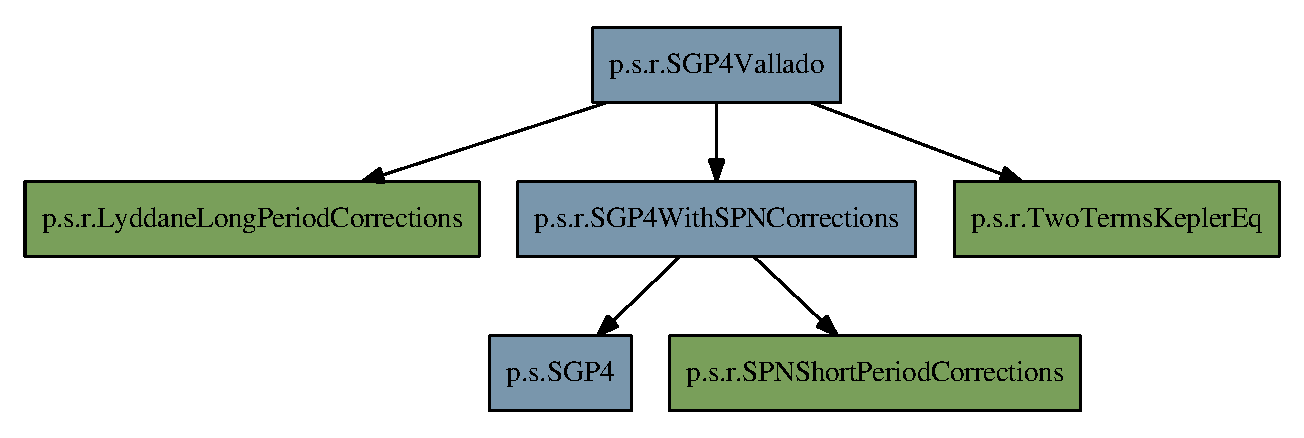
\includegraphics[width=\linewidth]{vallado.eps}
\caption{Structure of SGP4Vallado algorithm}
\label{fig:valladoeps}
\end{figure*}

\begin{figure}[htb]
  \centering
	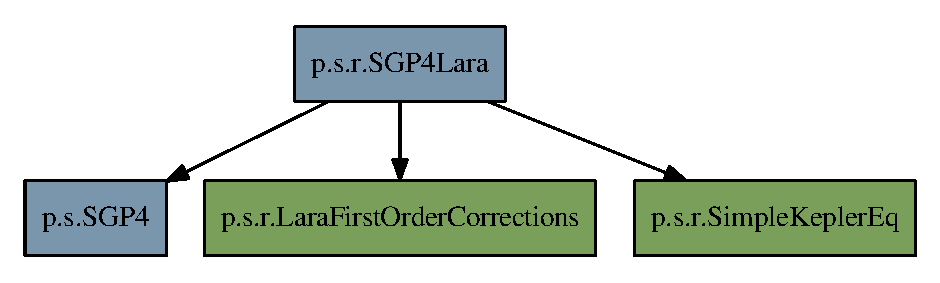
\includegraphics[width=\linewidth]{lara.eps}
\caption{Structure of SGP4Lara algorithm}
\label{fig:laraeps}
\end{figure}

%[{\color{red}Check that Figs.~(\ref{fig:res}) and (\ref{fig:res0}) are properly cited in the final version of the text}]


\section{SGP4 ALGORITHM DESCRIPTIONS}
\label{sec:algorithms}

The SGP4 propagator is thoroughly described in the literature \cite{HootsRoehrich1980,ValladoCrawfordHujsakKelso2006}. For completeness, we summarize it here, yet without mentioning anything related to the deep space or atmospheric drag corrections.

First, we recall that Brouwer's gravitational theory relies on the canonical set of Delaunay variables
\begin{itemize} \itemsep0em
\item $\ell=M$: mean anomaly
\item $g=\omega$: argument of the periapsis
\item $h=\Omega$: RAAN (right ascension of the ascending node)
\item $L=\sqrt{\mu\,a}$: Delaunay action, where $\mu$ is the earth gravitational constant and $a$ is the orbit semi-major axis
\item $G=\sqrt{\mu\,p}$: total angular momentum, where $p=a(1-e^2)$ is the orbit parameter (\textit{semilatus rectum}), and $e$ is the orbit eccentricity
\item $H=G\cos{I}$: projection of the angular momentum on the earth's rotation axis, where $I$ is the orbit inclination
\end{itemize}
However, Brouwer's theory finds trouble when evaluating the short-period corrections for the lower eccentricity orbits. The trouble is artificial, and is related to the singularity of Delaunay variables for circular orbits. Hence,
SGP4 implements a different set of elements based on Lyddane's approach which completely avoids that trouble. In particular, the elements used in the computation of short-period corrections are\footnote{The original variables proposed by Lyddane were slightly different, namely $a$, $F$, $e\cos\ell$, $e\sin\ell$, $\sin\frac{1}{2}I\cos{h}$, and $\sin\frac{1}{2}I\sin{h}$. }
\[
F=\ell+g+h, \quad C=e\cos\omega, \quad S=e\sin\omega, \quad a, \quad I, \quad h.
\]

\subsection{Standard implementation of SGP4} \label{sec:vallado}

\subsubsection{Initialization and secular corrections}
The code, starts from the initial mean elements at epoch $(I_0,\Omega_0,e_0,\omega_0,M_0,n_0)$, where $n$ stands for mean motion, which should be obtained from the so called two line elements, or TLEs.\footnote{Keep in mind that the TLE mean motion needs to be converted first from Kozai's definition \cite{Kozai1959} to Brouwer's secular one.} From them, Delaunay elements at epoch $(\ell_0'',g_0'', h_0'',L_0'',G_0'',H_0'')$ are obtained from their definition. The double prime notation is used for ``secular'' elements. In fact, the Delaunay actions, viz.~$L$, $G$, and $H$, are never computed in SGP4, which uses $n=\mu^2/L^3$, $e=\sqrt{1-G^2/L^2}$, and $I=\arccos(H/G)$, instead.

From these initial elements, Brouwer's theory provides the secular frequencies $\dot\ell''$, $\dot{g}''$, and $\dot{h}''$, due to the earth's gravitational potential, where the overdot means time derivative. Each of these frequencies is a function of $(n_0,e_0,I_0)$, and remain constant for the evaluation of the theory at different dates. Besides, the initialization process provides a series of coefficients needed to apply drag secular corrections as computed from Lane's theory \cite{Lane1965}.
\par

The code works with internal units of length $\mathrm{LU}$ (units of earth's radius $R_\oplus$ in km) and time $\mathrm{TU}$ (units of the orbit's period in min) such that $\mu=1\,\mathrm{LU^3/TU^2}$ in internal units. Besides, the expansion of the gravitational potential in SGP4 is limited to the (unnormalized) zonal harmonics $J_2$, $J_3$, and $J_4$. This selection of units helps in optimizing the code, but it is irrelevant for the description of the algorithms. Therefore, following descriptions include explicitly both the earth's gravitational parameter as well as the earth's equatorial radius.

The next step is to update the secular elements at epoch to the desired date given by the time $t$.

Brouwer's gravitational corrections are applied first
\[
\ell''_j=M_0+\dot\ell''\,t, \quad g''_j=\omega_0+\dot{g}''\,t, \quad h''_j=\Omega_0+\dot{h}''\,t, %\qquad L''_j=L_0, \quad G''_j=G_0, \quad H''=H_0
\]
where the subindex $j$ stands for gravitational effects only. Besides, corrections due to the atmospheric drag, which are not discussed in the paper, are incorporated at this stage.

After that, we obtain the set of secular elements
\[
(\ell'',g'',h'',a'',e'',I'').
\]
The secular mean motion $n''=(\mu/a''^3)^{1/2}$ is also computed.

\subsubsection{Geopotential periodic corrections} \label{s:SGP4lp}

Brouwer long-period gravitational corrections are reformulated in Lyddane's variables. At the precision of SGP4, that is, neglecting terms $\mathcal{O}(e^2)$, there are only corrections for $F$ and $S$. Then, $C'= C''$, $a'=a''$, $h'=h''$, $I'=I''$, and
\begin{eqnarray*}
F' &=& (\ell''+g''+h'')-\frac{J_3}{4J_2}\frac{R_\oplus}{p''}C''\frac{3+5\cos{I}''}{1+\cos{I}''}\sin{I}'' \\
S' &=&  e''\sin{g}'' -\frac{J_3}{2J_2}\frac{R_\oplus}{p''}\sin{I}''
\end{eqnarray*}
where $C''=e''\cos{g}''$, $p''=a''(1-e''^2)$. The single prime notation means that Lyddane elements include long-period effects. Note that $n'=n''$. Since there is no risk of ambiguity, the notation can be unified and simplified by removing primes, to read
%{\color{blue}The corresponding expression after unifying variables and removing primes is:
\begin{eqnarray*}
F &=&  M + \omega + \Omega - \epsilon_3 s e \cos{\omega}\frac{3+5c}{2(1+c)} \\
S &=& e\sin{\omega} - \epsilon_3 s
\end{eqnarray*}
where $c=\cos{I}$, $s=\sin{I}$, and $\epsilon_3=\frac{1}{2}(J_3/J_2)(R_\oplus/p)$.
%}

It follows a change from Lyddane's to polar variables
\[
(r,\theta,R=\dot{r},\Theta=r^2\dot\theta)\longrightarrow(F,C,S,a).
\]
To do that, first the Kepler equation
\[
U\equiv{F'-h'}=\Psi+S'\cos\Psi-C'\sin\Psi,
\]
is solved to compute $\Psi=E'+g'$, where $E$ is the eccentric anomaly. Newton-Raphson iterations start from $\Psi_0=U$.

Next $g'$ and $e'$ are solved from $C'=e'\cos{g'}$, $S'=e'\sin{g}'$. Then, compute $E'=\Psi-g'$, $L'=\sqrt{\mu{a}'}$, and $\beta'=\sqrt{1-e'^2}$. It follows the usual transformation
\begin{eqnarray} \label{eq:utor}
r' &=& a'(1-e'\cos{E}') \\
R' &=& (L'/r')e'\sin{E}' \\
\Theta' &=& L'\beta' \\
\theta' &=& f'+g'
\end{eqnarray}
where the true anomaly is obtained without ambiguity from
\begin{equation} \label{eq:utof}
\sin{f}'=(a'/r')\beta'\sin{E}',\quad \cos{f}'=(a'/r')(\cos{E}'-e').
\end{equation}
Note that, SGP4 computes the correction to $r\dot\theta=\Theta/r$ instead of the correction to the polar variable $\Theta$.


% \subsubsection{Short-period gravitational corrections}
Then, compute $p'=a'\beta'^2$, $c'=\cos{I}'$, $s'=\sin{I}'$, and $\epsilon_2=-\frac{1}{4}J_2(R_\oplus/p')^2$, to obtain the SGP4 short-period corrections
\begin{eqnarray*}
\delta r &=& \epsilon_2\left[3\beta'r'(3c'^2-1)-p's'^2\cos2\theta'\right] \\
\delta \theta &=& \frac{1}{2}\epsilon_2(7c'^2-1)\sin{2\theta'} \\
\delta \Omega &=& -3\epsilon_2 c'\sin2\theta' \\
\delta R &=& 2\epsilon_2 p'n's'^2\sin2\theta' \\
\delta I &=& -3\epsilon_2 c'\,s'\cos2\theta' \\
\delta \frac{\Theta}{r} &=&
- \epsilon_2\frac{\Theta'}{p'}\left[2s'^2\cos2\theta'+3\left(3c'^2-1\right)\right]
\end{eqnarray*}
which neglect terms of $\mathcal{O}(e)$.


Finally, the state vector is computed from the standard transformation from Cartesian to polar-nodal variables
\[ %\begin{equation} \label{Kepler:Whittaker}
\left(\begin{array}{cc} x & \dot{x} \\ y & \dot{y} \\ z & \dot{z} \end{array}\right)=
R_3(-\Omega)\,{R}_1(-I)\,{R}_3(-\theta)\,\left(\begin{array}{cc} r & R \\ 0 & \Theta/r \\ 0 & 0 \end{array}\right)
\] %\end{equation}
where $R_1$ and $R_3$ are the usual rotation matrices about the $x$ and $z$ axes, respectively


\subsection{Lara's algorithm in non-singular variables} \label{sec:lara}

A straightforward alternative to the SGP4 implementation is to proceed in Lara's non-singular variables \cite{Lara2015MPE} both for the long- and short-period gravitational corrections. The modifications to the SGP4 algorithm start from Section \ref{s:SGP4lp} as follows.

Now, Kepler equation $\ell''=E''-e''\sin{E}''$ must be solved first to compute the (secular) eccentric anomaly, and then the (secular) true anomaly
\[
f''=2\arctan\left(\sqrt{\frac{1+e''}{1-e''}}\tan\frac{E''}{2}\right).
\]
\par

Next, Delaunay variables are transformed to polar variables using the same equations as Eqs.~(\ref{eq:utor})--(\ref{eq:utof}) but now with double prime variables, which in turn are transformed to Lara's non-singular variables
%$\psi=\theta+h$, $\xi=\sin{I}\sin\theta$, $\chi=\sin{I}\cos\theta$, $r$, $R$, $\Theta$
\[
\psi=\theta+\Omega,\quad \xi=\sin{I}\sin\theta,\quad \chi=\sin{I}\cos\theta,\quad r,\; R,\; \Theta.
\]


Then, apply the long-period corrections
\begin{eqnarray*} \label{eq:dyns}
\delta\psi &=& \epsilon_3\left[2 \chi+(\kappa  \chi -c \xi  \sigma)/(1+c)\right],
\\  \label{eq:dxins}
\delta\xi &=&
\epsilon_3\left[2 \chi ^2+\kappa  \left(1-\xi ^2\right) \right],
\\ \label{eq:dchins}
\delta\chi &=& %-2\epsilon_3\,\chi\,\xi=
-\epsilon_3\left[c^2 \sigma +(2+\kappa) \xi  \chi \right],
\\ \label{eq:drns}
\delta{r} &=& \epsilon_3\,\xi\,p,
\\ \label{eq:dRRns}
\delta{R} &=& % ({\Theta}/{p})\,\epsilon_3\,\chi=
\epsilon_3\,(1+\kappa)\,\chi\,\Theta/r,
\\ \label{eq:dZZns}
\delta\Theta &=&\epsilon_3(\kappa\xi-\sigma\chi)\,\Theta,
%\\ \label{eq:dNNns} \color{red}
%\delta{N} &=& 0,
\end{eqnarray*}
where $c=\sqrt{1-\xi^2-\chi^2}$, $\kappa=-1+p/r$, $\sigma=pR/\Theta$, and $p=\Theta^2/\mu$. Note that this corrections have no contributions of $\mathcal{O}(e^2)$ and, therefore, do not accept any simplification at the precision of SGP4. The notation has been simplified avoiding primes because there is no risk of confusion.
\par


It follows the computation of the short-period corrections
\begin{eqnarray*} \label{lspc}
\Delta\psi &=& -\epsilon_2\frac{1+7c}{1+c}\,\xi\,\chi
\\
\Delta\xi &=& -\epsilon_2\left(\chi^2-3c^2\right)\xi
\\[1ex]
\Delta\chi &=& \epsilon_2\left(\xi^2-3c^2\right)\chi
\\
\Delta{r} &=& % \epsilon_2p\left[(\xi^2-\chi^2)-3(1-3c^2)\right]=
2\epsilon_2r\left(\xi^2-2+5c^2\right)
\\
\Delta{R} &=& %4\epsilon_2\,(\Theta/p)\xi\,\chi=
4\epsilon_2\,(\Theta/r)\xi\,\chi
\\
\Delta\Theta &=&  3\epsilon_2\,\Theta(\xi^2-\chi^2)
\end{eqnarray*}
where $c=\cos{I}$, $s=\sin{I}$, and $\epsilon_2=-\frac{1}{4}(R_\oplus/p)^2J_2$, which have been simplifyed neglecting terms of $\mathcal{O}(e)$ according to SGP4 criteria.
\par

Finally, the state vector is computed from
\begin{eqnarray*} \label{eq:ns2x}
x &=& r\,(b\cos\psi+q\sin\psi) \\ \label{eq:ns2y}
y &=& r\,(b\sin\psi-q\cos\psi) \\
z &=& r\,\xi \\
X &=& x\,(R/r) %(b\cos\psi+q\sin\psi)
 - ({\Theta}/{r})\,(q\cos\psi+\tau\sin\psi) \\ \label{eq:ns2Y}
Y &=& y\,(R/r) %(b\sin\psi-q\cos\psi)
 - ({\Theta}/{r})\,(q\sin\psi-\tau\cos\psi) \\  \label{eq:ns2zz}
Z &=& z\,(R/r)+(\Theta/r)\,\chi
\end{eqnarray*}
where
\[%\begin{equation} \label{tq}
b=1-\frac{\xi^2}{1+c}, \qquad
\tau=1 - \frac{\chi^2}{1 + c}, \qquad
q=\frac{\xi\,\chi}{1+c},
\]%\end{equation}
and $c=H/\Theta$. Remark that $H$ is an integral of the zonal problem and, therefore, its value is always known from given initial conditions $H=H_0''$.

% TODO: should we revise the Short Period Corrections in non-singular variables?
%       objective: better match in the plots


\section{VALIDATION}
\label{sec:validation}

The validation of the software has been done by comparing the results with those
of Vallado's original C++ source with propagations up to 3 weeks. The C++ source has been slightly modified in order
to save the cartesian coordinates, the unit vector, the polar nodals coordinates
and the long period corrections into a file. The modified sources and output file results are available as
well online at \\
\url{https://github.com/pleira/sgpvallado} \\
The outputs were collected for the Near Earth test cases detailed in Table \ref{tab:res}.

\begin{table*}[htb]
\centering
\caption{Near Earth TLEs used for testing}\vspace{2mm}
\begin{tabular}{ll}
\hline
Satellite & Comment \\
\hline
00005 & TEME example satellite.\\
06251 & Normal drag case, perigee 377.26 km.\\
22312 & Low perigee (86.98 km).\\
28057 & Normal drag case, low eccentricity (0.000 088 4).\\
28350 & Low perigee (127.20 km).\\
28872 & Perigee 51 km used to test error handling.\\
29141 & Last stages of decay.\\
29238 & Perigee 212.24 km, simplified drag branch.\\
\hline\hline
\end{tabular}
\label{tab:res}
\end{table*}

The results for the SGP4Vallado algorithm in Scala matches the C++ results with neglible differences for all test propagations (maximum differences of the order of 3E-8).

When propagating satellites 22312 and 28350, the SGP4-Vallado implementation went into error at an earlier time
than the C++ version because of the negative value for the eccentricity, being the times 454.2028672 versus 474.2028672 for 22312 and 960 versus 1440 for 28350.
For the satellite 28872, propagation with SGP4Vallado ends by epoch minute 50 as in Vallado's C++.

\subsection{Test for eccentric anomaly}
\label{sec:trueanomaly}

Lara's algorithm is done in non singular variables which are related to polar nodal variables.
To transform from classical secular elements to those non-singular variables, the eccentric anomaly has to be calculated first, as described in Section \ref{sec:lara}.
Vallado's algorithm does the calculation of the eccentric anomaly after the long period corrections have been applied using Lyddane's variables.
We have checked that, as expected, the order in which the eccentric anomaly is calculated has negligible effect in the long period corrections.

Two algorithms have been developed to test this fact, SGP4PN and SGP4ValladoLong.
SGP4PN does the calculation of long period corrections in polar nodal variables (SpecialPolarNodal in the code) and therefore requires
to calculate Kepler equation before the long period corrections as in SGP4Lara. SGP4PN includes the same terms for long period corrections as in SGP4Lara,
which include some more effects than those in SGP4Vallado. For the comparison, the SGP4ValladoLong algorithm includes the same long period effects expressed
in Lyddane's variables, that is, without neglecting long-period corrections of $\mathcal{O}(e^2)$ and higher, and afterwards, solves the Kepler equation as in SGP4Vallado.
The short period corrections for all SGP4Vallado, SGP4PN and SGP4ValladoLong share the same code expressed in polar nodals variables.
The results of comparing the output in polar nodals variables in internal units after the periodic corrections were calculated between SGP4ValladoLong and SGP4PN for propagations up to 3 weeks
gave maximum differences of the order 1.6E-6, which shows no significant effect introduced by the order of the calculation of the eccentric anomaly.

Figures (\ref{fig:pos05})--(\ref{fig:vel05}) show the comparison of propagation results for the test TLE 00005 for 1 day with SGP4Vallado (which correspond to Vallado's C++ results) to the other three different algorithms.
The inclusion of more terms in the long period corrections for the other algorithms produce differences.
SGP4PN and SGP4ValladoLong come displayed one a top the other, which shows no effect by the order in the calculation of the eccentric anomaly as mentioned previously.
Also, the differences between in the short period corrections between Lara and the rest of the algorithms account for the different behaviour of Lara's algorithm.

\begin{figure}[htb]
  % GNUPLOT: LaTeX picture with Postscript
\begingroup
  \makeatletter
  \providecommand\color[2][]{%
    \GenericError{(gnuplot) \space\space\space\@spaces}{%
      Package color not loaded in conjunction with
      terminal option `colourtext'%
    }{See the gnuplot documentation for explanation.%
    }{Either use 'blacktext' in gnuplot or load the package
      color.sty in LaTeX.}%
    \renewcommand\color[2][]{}%
  }%
  \providecommand\includegraphics[2][]{%
    \GenericError{(gnuplot) \space\space\space\@spaces}{%
      Package graphicx or graphics not loaded%
    }{See the gnuplot documentation for explanation.%
    }{The gnuplot epslatex terminal needs graphicx.sty or graphics.sty.}%
    \renewcommand\includegraphics[2][]{}%
  }%
  \providecommand\rotatebox[2]{#2}%
  \@ifundefined{ifGPcolor}{%
    \newif\ifGPcolor
    \GPcolortrue
  }{}%
  \@ifundefined{ifGPblacktext}{%
    \newif\ifGPblacktext
    \GPblacktextfalse
  }{}%
  % define a \g@addto@macro without @ in the name:
  \let\gplgaddtomacro\g@addto@macro
  % define empty templates for all commands taking text:
  \gdef\gplbacktext{}%
  \gdef\gplfronttext{}%
  \makeatother
  \ifGPblacktext
    % no textcolor at all
    \def\colorrgb#1{}%
    \def\colorgray#1{}%
  \else
    % gray or color?
    \ifGPcolor
      \def\colorrgb#1{\color[rgb]{#1}}%
      \def\colorgray#1{\color[gray]{#1}}%
      \expandafter\def\csname LTw\endcsname{\color{white}}%
      \expandafter\def\csname LTb\endcsname{\color{black}}%
      \expandafter\def\csname LTa\endcsname{\color{black}}%
      \expandafter\def\csname LT0\endcsname{\color[rgb]{1,0,0}}%
      \expandafter\def\csname LT1\endcsname{\color[rgb]{0,1,0}}%
      \expandafter\def\csname LT2\endcsname{\color[rgb]{0,0,1}}%
      \expandafter\def\csname LT3\endcsname{\color[rgb]{1,0,1}}%
      \expandafter\def\csname LT4\endcsname{\color[rgb]{0,1,1}}%
      \expandafter\def\csname LT5\endcsname{\color[rgb]{1,1,0}}%
      \expandafter\def\csname LT6\endcsname{\color[rgb]{0,0,0}}%
      \expandafter\def\csname LT7\endcsname{\color[rgb]{1,0.3,0}}%
      \expandafter\def\csname LT8\endcsname{\color[rgb]{0.5,0.5,0.5}}%
    \else
      % gray
      \def\colorrgb#1{\color{black}}%
      \def\colorgray#1{\color[gray]{#1}}%
      \expandafter\def\csname LTw\endcsname{\color{white}}%
      \expandafter\def\csname LTb\endcsname{\color{black}}%
      \expandafter\def\csname LTa\endcsname{\color{black}}%
      \expandafter\def\csname LT0\endcsname{\color{black}}%
      \expandafter\def\csname LT1\endcsname{\color{black}}%
      \expandafter\def\csname LT2\endcsname{\color{black}}%
      \expandafter\def\csname LT3\endcsname{\color{black}}%
      \expandafter\def\csname LT4\endcsname{\color{black}}%
      \expandafter\def\csname LT5\endcsname{\color{black}}%
      \expandafter\def\csname LT6\endcsname{\color{black}}%
      \expandafter\def\csname LT7\endcsname{\color{black}}%
      \expandafter\def\csname LT8\endcsname{\color{black}}%
    \fi
  \fi
  \setlength{\unitlength}{0.0500bp}%
  \begin{picture}(5040.00,3770.00)%
    \gplgaddtomacro\gplbacktext{%
      \csname LTb\endcsname%
      \put(946,704){\makebox(0,0)[r]{\strut{}$-0.5$}}%
      \put(946,1104){\makebox(0,0)[r]{\strut{}$-0.4$}}%
      \put(946,1504){\makebox(0,0)[r]{\strut{}$-0.3$}}%
      \put(946,1904){\makebox(0,0)[r]{\strut{}$-0.2$}}%
      \put(946,2305){\makebox(0,0)[r]{\strut{}$-0.1$}}%
      \put(946,2705){\makebox(0,0)[r]{\strut{}$0$}}%
      \put(946,3105){\makebox(0,0)[r]{\strut{}$0.1$}}%
      \put(946,3505){\makebox(0,0)[r]{\strut{}$0.2$}}%
      \put(1078,484){\makebox(0,0){\strut{}$0$}}%
      \put(1474,484){\makebox(0,0){\strut{}$50$}}%
      \put(1870,484){\makebox(0,0){\strut{}$100$}}%
      \put(2266,484){\makebox(0,0){\strut{}$150$}}%
      \put(2662,484){\makebox(0,0){\strut{}$200$}}%
      \put(3059,484){\makebox(0,0){\strut{}$250$}}%
      \put(3455,484){\makebox(0,0){\strut{}$300$}}%
      \put(3851,484){\makebox(0,0){\strut{}$350$}}%
      \put(4247,484){\makebox(0,0){\strut{}$400$}}%
      \put(4643,484){\makebox(0,0){\strut{}$450$}}%
      \put(176,2104){\rotatebox{-270}{\makebox(0,0){\strut{}$Difference (km)$}}}%
      \put(2860,154){\makebox(0,0){\strut{}$Minutes$}}%
    }%
    \gplgaddtomacro\gplfronttext{%
      \csname LTb\endcsname%
      \put(1474,3332){\makebox(0,0)[r]{\strut{}vl}}%
      \csname LTb\endcsname%
      \put(1474,3112){\makebox(0,0)[r]{\strut{}pn}}%
      \csname LTb\endcsname%
      \put(1474,2892){\makebox(0,0)[r]{\strut{}la}}%
    }%
    \gplbacktext
    \put(0,0){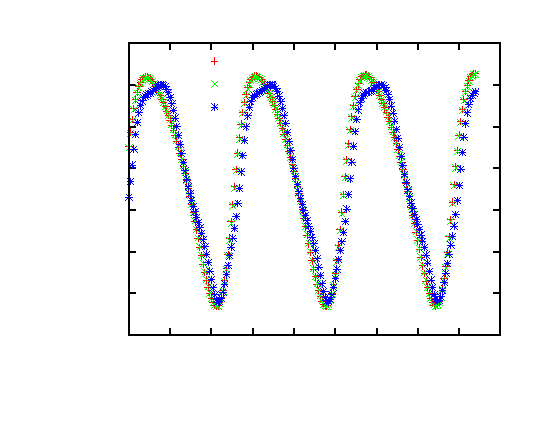
\includegraphics{dx_cartesian_00005}}%
    \gplfronttext
  \end{picture}%
\endgroup

  % GNUPLOT: LaTeX picture with Postscript
\begingroup
  \makeatletter
  \providecommand\color[2][]{%
    \GenericError{(gnuplot) \space\space\space\@spaces}{%
      Package color not loaded in conjunction with
      terminal option `colourtext'%
    }{See the gnuplot documentation for explanation.%
    }{Either use 'blacktext' in gnuplot or load the package
      color.sty in LaTeX.}%
    \renewcommand\color[2][]{}%
  }%
  \providecommand\includegraphics[2][]{%
    \GenericError{(gnuplot) \space\space\space\@spaces}{%
      Package graphicx or graphics not loaded%
    }{See the gnuplot documentation for explanation.%
    }{The gnuplot epslatex terminal needs graphicx.sty or graphics.sty.}%
    \renewcommand\includegraphics[2][]{}%
  }%
  \providecommand\rotatebox[2]{#2}%
  \@ifundefined{ifGPcolor}{%
    \newif\ifGPcolor
    \GPcolortrue
  }{}%
  \@ifundefined{ifGPblacktext}{%
    \newif\ifGPblacktext
    \GPblacktextfalse
  }{}%
  % define a \g@addto@macro without @ in the name:
  \let\gplgaddtomacro\g@addto@macro
  % define empty templates for all commands taking text:
  \gdef\gplbacktext{}%
  \gdef\gplfronttext{}%
  \makeatother
  \ifGPblacktext
    % no textcolor at all
    \def\colorrgb#1{}%
    \def\colorgray#1{}%
  \else
    % gray or color?
    \ifGPcolor
      \def\colorrgb#1{\color[rgb]{#1}}%
      \def\colorgray#1{\color[gray]{#1}}%
      \expandafter\def\csname LTw\endcsname{\color{white}}%
      \expandafter\def\csname LTb\endcsname{\color{black}}%
      \expandafter\def\csname LTa\endcsname{\color{black}}%
      \expandafter\def\csname LT0\endcsname{\color[rgb]{1,0,0}}%
      \expandafter\def\csname LT1\endcsname{\color[rgb]{0,1,0}}%
      \expandafter\def\csname LT2\endcsname{\color[rgb]{0,0,1}}%
      \expandafter\def\csname LT3\endcsname{\color[rgb]{1,0,1}}%
      \expandafter\def\csname LT4\endcsname{\color[rgb]{0,1,1}}%
      \expandafter\def\csname LT5\endcsname{\color[rgb]{1,1,0}}%
      \expandafter\def\csname LT6\endcsname{\color[rgb]{0,0,0}}%
      \expandafter\def\csname LT7\endcsname{\color[rgb]{1,0.3,0}}%
      \expandafter\def\csname LT8\endcsname{\color[rgb]{0.5,0.5,0.5}}%
    \else
      % gray
      \def\colorrgb#1{\color{black}}%
      \def\colorgray#1{\color[gray]{#1}}%
      \expandafter\def\csname LTw\endcsname{\color{white}}%
      \expandafter\def\csname LTb\endcsname{\color{black}}%
      \expandafter\def\csname LTa\endcsname{\color{black}}%
      \expandafter\def\csname LT0\endcsname{\color{black}}%
      \expandafter\def\csname LT1\endcsname{\color{black}}%
      \expandafter\def\csname LT2\endcsname{\color{black}}%
      \expandafter\def\csname LT3\endcsname{\color{black}}%
      \expandafter\def\csname LT4\endcsname{\color{black}}%
      \expandafter\def\csname LT5\endcsname{\color{black}}%
      \expandafter\def\csname LT6\endcsname{\color{black}}%
      \expandafter\def\csname LT7\endcsname{\color{black}}%
      \expandafter\def\csname LT8\endcsname{\color{black}}%
    \fi
  \fi
  \setlength{\unitlength}{0.0500bp}%
  \begin{picture}(5040.00,3770.00)%
    \gplgaddtomacro\gplbacktext{%
      \csname LTb\endcsname%
      \put(946,704){\makebox(0,0)[r]{\strut{}$-0.8$}}%
      \put(946,1104){\makebox(0,0)[r]{\strut{}$-0.6$}}%
      \put(946,1504){\makebox(0,0)[r]{\strut{}$-0.4$}}%
      \put(946,1904){\makebox(0,0)[r]{\strut{}$-0.2$}}%
      \put(946,2305){\makebox(0,0)[r]{\strut{}$0$}}%
      \put(946,2705){\makebox(0,0)[r]{\strut{}$0.2$}}%
      \put(946,3105){\makebox(0,0)[r]{\strut{}$0.4$}}%
      \put(946,3505){\makebox(0,0)[r]{\strut{}$0.6$}}%
      \put(1078,484){\makebox(0,0){\strut{}$0$}}%
      \put(1474,484){\makebox(0,0){\strut{}$50$}}%
      \put(1870,484){\makebox(0,0){\strut{}$100$}}%
      \put(2266,484){\makebox(0,0){\strut{}$150$}}%
      \put(2662,484){\makebox(0,0){\strut{}$200$}}%
      \put(3059,484){\makebox(0,0){\strut{}$250$}}%
      \put(3455,484){\makebox(0,0){\strut{}$300$}}%
      \put(3851,484){\makebox(0,0){\strut{}$350$}}%
      \put(4247,484){\makebox(0,0){\strut{}$400$}}%
      \put(4643,484){\makebox(0,0){\strut{}$450$}}%
      \put(176,2104){\rotatebox{-270}{\makebox(0,0){\strut{}$Difference (km)$}}}%
      \put(2860,154){\makebox(0,0){\strut{}$Minutes$}}%
    }%
    \gplgaddtomacro\gplfronttext{%
      \csname LTb\endcsname%
      \put(1474,3332){\makebox(0,0)[r]{\strut{}vl}}%
      \csname LTb\endcsname%
      \put(1474,3112){\makebox(0,0)[r]{\strut{}pn}}%
      \csname LTb\endcsname%
      \put(1474,2892){\makebox(0,0)[r]{\strut{}la}}%
    }%
    \gplbacktext
    \put(0,0){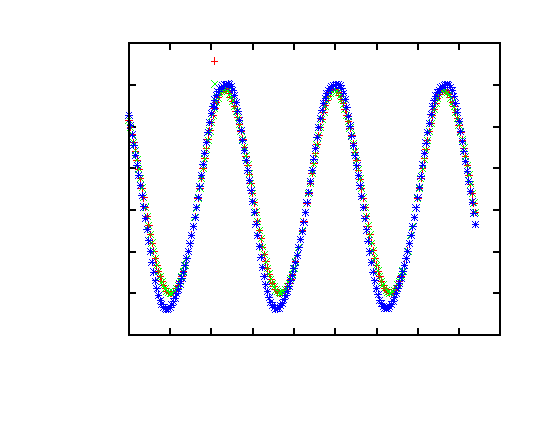
\includegraphics{dy_cartesian_00005}}%
    \gplfronttext
  \end{picture}%
\endgroup

  % GNUPLOT: LaTeX picture with Postscript
\begingroup
  \makeatletter
  \providecommand\color[2][]{%
    \GenericError{(gnuplot) \space\space\space\@spaces}{%
      Package color not loaded in conjunction with
      terminal option `colourtext'%
    }{See the gnuplot documentation for explanation.%
    }{Either use 'blacktext' in gnuplot or load the package
      color.sty in LaTeX.}%
    \renewcommand\color[2][]{}%
  }%
  \providecommand\includegraphics[2][]{%
    \GenericError{(gnuplot) \space\space\space\@spaces}{%
      Package graphicx or graphics not loaded%
    }{See the gnuplot documentation for explanation.%
    }{The gnuplot epslatex terminal needs graphicx.sty or graphics.sty.}%
    \renewcommand\includegraphics[2][]{}%
  }%
  \providecommand\rotatebox[2]{#2}%
  \@ifundefined{ifGPcolor}{%
    \newif\ifGPcolor
    \GPcolortrue
  }{}%
  \@ifundefined{ifGPblacktext}{%
    \newif\ifGPblacktext
    \GPblacktextfalse
  }{}%
  % define a \g@addto@macro without @ in the name:
  \let\gplgaddtomacro\g@addto@macro
  % define empty templates for all commands taking text:
  \gdef\gplbacktext{}%
  \gdef\gplfronttext{}%
  \makeatother
  \ifGPblacktext
    % no textcolor at all
    \def\colorrgb#1{}%
    \def\colorgray#1{}%
  \else
    % gray or color?
    \ifGPcolor
      \def\colorrgb#1{\color[rgb]{#1}}%
      \def\colorgray#1{\color[gray]{#1}}%
      \expandafter\def\csname LTw\endcsname{\color{white}}%
      \expandafter\def\csname LTb\endcsname{\color{black}}%
      \expandafter\def\csname LTa\endcsname{\color{black}}%
      \expandafter\def\csname LT0\endcsname{\color[rgb]{1,0,0}}%
      \expandafter\def\csname LT1\endcsname{\color[rgb]{0,1,0}}%
      \expandafter\def\csname LT2\endcsname{\color[rgb]{0,0,1}}%
      \expandafter\def\csname LT3\endcsname{\color[rgb]{1,0,1}}%
      \expandafter\def\csname LT4\endcsname{\color[rgb]{0,1,1}}%
      \expandafter\def\csname LT5\endcsname{\color[rgb]{1,1,0}}%
      \expandafter\def\csname LT6\endcsname{\color[rgb]{0,0,0}}%
      \expandafter\def\csname LT7\endcsname{\color[rgb]{1,0.3,0}}%
      \expandafter\def\csname LT8\endcsname{\color[rgb]{0.5,0.5,0.5}}%
    \else
      % gray
      \def\colorrgb#1{\color{black}}%
      \def\colorgray#1{\color[gray]{#1}}%
      \expandafter\def\csname LTw\endcsname{\color{white}}%
      \expandafter\def\csname LTb\endcsname{\color{black}}%
      \expandafter\def\csname LTa\endcsname{\color{black}}%
      \expandafter\def\csname LT0\endcsname{\color{black}}%
      \expandafter\def\csname LT1\endcsname{\color{black}}%
      \expandafter\def\csname LT2\endcsname{\color{black}}%
      \expandafter\def\csname LT3\endcsname{\color{black}}%
      \expandafter\def\csname LT4\endcsname{\color{black}}%
      \expandafter\def\csname LT5\endcsname{\color{black}}%
      \expandafter\def\csname LT6\endcsname{\color{black}}%
      \expandafter\def\csname LT7\endcsname{\color{black}}%
      \expandafter\def\csname LT8\endcsname{\color{black}}%
    \fi
  \fi
  \setlength{\unitlength}{0.0500bp}%
  \begin{picture}(5040.00,3770.00)%
    \gplgaddtomacro\gplbacktext{%
      \csname LTb\endcsname%
      \put(946,704){\makebox(0,0)[r]{\strut{}$-1$}}%
      \put(946,1264){\makebox(0,0)[r]{\strut{}$-0.5$}}%
      \put(946,1824){\makebox(0,0)[r]{\strut{}$0$}}%
      \put(946,2385){\makebox(0,0)[r]{\strut{}$0.5$}}%
      \put(946,2945){\makebox(0,0)[r]{\strut{}$1$}}%
      \put(946,3505){\makebox(0,0)[r]{\strut{}$1.5$}}%
      \put(1078,484){\makebox(0,0){\strut{}$0$}}%
      \put(1474,484){\makebox(0,0){\strut{}$50$}}%
      \put(1870,484){\makebox(0,0){\strut{}$100$}}%
      \put(2266,484){\makebox(0,0){\strut{}$150$}}%
      \put(2662,484){\makebox(0,0){\strut{}$200$}}%
      \put(3059,484){\makebox(0,0){\strut{}$250$}}%
      \put(3455,484){\makebox(0,0){\strut{}$300$}}%
      \put(3851,484){\makebox(0,0){\strut{}$350$}}%
      \put(4247,484){\makebox(0,0){\strut{}$400$}}%
      \put(4643,484){\makebox(0,0){\strut{}$450$}}%
      \put(176,2104){\rotatebox{-270}{\makebox(0,0){\strut{}$Difference (km)$}}}%
      \put(2860,154){\makebox(0,0){\strut{}$Minutes$}}%
    }%
    \gplgaddtomacro\gplfronttext{%
      \csname LTb\endcsname%
      \put(1474,3332){\makebox(0,0)[r]{\strut{}vl}}%
      \csname LTb\endcsname%
      \put(1474,3112){\makebox(0,0)[r]{\strut{}pn}}%
      \csname LTb\endcsname%
      \put(1474,2892){\makebox(0,0)[r]{\strut{}la}}%
    }%
    \gplbacktext
    \put(0,0){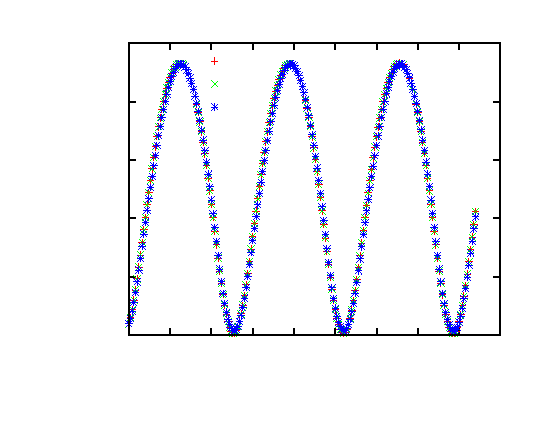
\includegraphics{dz_cartesian_00005}}%
    \gplfronttext
  \end{picture}%
\endgroup

\caption{Difference (km) of SGP4Extension algorithms Lara, Vallado Long and Polar Nodals with Vallado's C++ results for TLE 00005}
\label{fig:pos05}
\end{figure}


\begin{figure}[htb]
  % GNUPLOT: LaTeX picture with Postscript
\begingroup
  \makeatletter
  \providecommand\color[2][]{%
    \GenericError{(gnuplot) \space\space\space\@spaces}{%
      Package color not loaded in conjunction with
      terminal option `colourtext'%
    }{See the gnuplot documentation for explanation.%
    }{Either use 'blacktext' in gnuplot or load the package
      color.sty in LaTeX.}%
    \renewcommand\color[2][]{}%
  }%
  \providecommand\includegraphics[2][]{%
    \GenericError{(gnuplot) \space\space\space\@spaces}{%
      Package graphicx or graphics not loaded%
    }{See the gnuplot documentation for explanation.%
    }{The gnuplot epslatex terminal needs graphicx.sty or graphics.sty.}%
    \renewcommand\includegraphics[2][]{}%
  }%
  \providecommand\rotatebox[2]{#2}%
  \@ifundefined{ifGPcolor}{%
    \newif\ifGPcolor
    \GPcolortrue
  }{}%
  \@ifundefined{ifGPblacktext}{%
    \newif\ifGPblacktext
    \GPblacktextfalse
  }{}%
  % define a \g@addto@macro without @ in the name:
  \let\gplgaddtomacro\g@addto@macro
  % define empty templates for all commands taking text:
  \gdef\gplbacktext{}%
  \gdef\gplfronttext{}%
  \makeatother
  \ifGPblacktext
    % no textcolor at all
    \def\colorrgb#1{}%
    \def\colorgray#1{}%
  \else
    % gray or color?
    \ifGPcolor
      \def\colorrgb#1{\color[rgb]{#1}}%
      \def\colorgray#1{\color[gray]{#1}}%
      \expandafter\def\csname LTw\endcsname{\color{white}}%
      \expandafter\def\csname LTb\endcsname{\color{black}}%
      \expandafter\def\csname LTa\endcsname{\color{black}}%
      \expandafter\def\csname LT0\endcsname{\color[rgb]{1,0,0}}%
      \expandafter\def\csname LT1\endcsname{\color[rgb]{0,1,0}}%
      \expandafter\def\csname LT2\endcsname{\color[rgb]{0,0,1}}%
      \expandafter\def\csname LT3\endcsname{\color[rgb]{1,0,1}}%
      \expandafter\def\csname LT4\endcsname{\color[rgb]{0,1,1}}%
      \expandafter\def\csname LT5\endcsname{\color[rgb]{1,1,0}}%
      \expandafter\def\csname LT6\endcsname{\color[rgb]{0,0,0}}%
      \expandafter\def\csname LT7\endcsname{\color[rgb]{1,0.3,0}}%
      \expandafter\def\csname LT8\endcsname{\color[rgb]{0.5,0.5,0.5}}%
    \else
      % gray
      \def\colorrgb#1{\color{black}}%
      \def\colorgray#1{\color[gray]{#1}}%
      \expandafter\def\csname LTw\endcsname{\color{white}}%
      \expandafter\def\csname LTb\endcsname{\color{black}}%
      \expandafter\def\csname LTa\endcsname{\color{black}}%
      \expandafter\def\csname LT0\endcsname{\color{black}}%
      \expandafter\def\csname LT1\endcsname{\color{black}}%
      \expandafter\def\csname LT2\endcsname{\color{black}}%
      \expandafter\def\csname LT3\endcsname{\color{black}}%
      \expandafter\def\csname LT4\endcsname{\color{black}}%
      \expandafter\def\csname LT5\endcsname{\color{black}}%
      \expandafter\def\csname LT6\endcsname{\color{black}}%
      \expandafter\def\csname LT7\endcsname{\color{black}}%
      \expandafter\def\csname LT8\endcsname{\color{black}}%
    \fi
  \fi
  \setlength{\unitlength}{0.0500bp}%
  \begin{picture}(5040.00,3770.00)%
    \gplgaddtomacro\gplbacktext{%
      \csname LTb\endcsname%
      \put(1342,704){\makebox(0,0)[r]{\strut{}$-0.0004$}}%
      \put(1342,1054){\makebox(0,0)[r]{\strut{}$-0.0002$}}%
      \put(1342,1404){\makebox(0,0)[r]{\strut{}$0$}}%
      \put(1342,1754){\makebox(0,0)[r]{\strut{}$0.0002$}}%
      \put(1342,2105){\makebox(0,0)[r]{\strut{}$0.0004$}}%
      \put(1342,2455){\makebox(0,0)[r]{\strut{}$0.0006$}}%
      \put(1342,2805){\makebox(0,0)[r]{\strut{}$0.0008$}}%
      \put(1342,3155){\makebox(0,0)[r]{\strut{}$0.001$}}%
      \put(1342,3505){\makebox(0,0)[r]{\strut{}$0.0012$}}%
      \put(1474,484){\makebox(0,0){\strut{}$0$}}%
      \put(1826,484){\makebox(0,0){\strut{}$50$}}%
      \put(2178,484){\makebox(0,0){\strut{}$100$}}%
      \put(2530,484){\makebox(0,0){\strut{}$150$}}%
      \put(2882,484){\makebox(0,0){\strut{}$200$}}%
      \put(3235,484){\makebox(0,0){\strut{}$250$}}%
      \put(3587,484){\makebox(0,0){\strut{}$300$}}%
      \put(3939,484){\makebox(0,0){\strut{}$350$}}%
      \put(4291,484){\makebox(0,0){\strut{}$400$}}%
      \put(4643,484){\makebox(0,0){\strut{}$450$}}%
      \put(176,2104){\rotatebox{-270}{\makebox(0,0){\strut{}$Difference (km/s)$}}}%
      \put(3058,154){\makebox(0,0){\strut{}$Minutes$}}%
    }%
    \gplgaddtomacro\gplfronttext{%
      \csname LTb\endcsname%
      \put(1870,3332){\makebox(0,0)[r]{\strut{}vl}}%
      \csname LTb\endcsname%
      \put(1870,3112){\makebox(0,0)[r]{\strut{}pn}}%
      \csname LTb\endcsname%
      \put(1870,2892){\makebox(0,0)[r]{\strut{}la}}%
    }%
    \gplbacktext
    \put(0,0){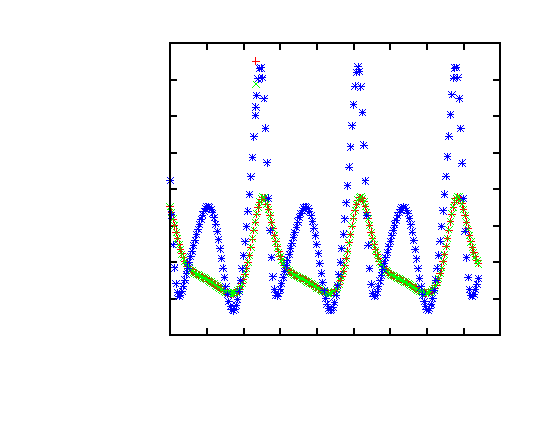
\includegraphics{dvx_cartesian_00005}}%
    \gplfronttext
  \end{picture}%
\endgroup

  % GNUPLOT: LaTeX picture with Postscript
\begingroup
  \makeatletter
  \providecommand\color[2][]{%
    \GenericError{(gnuplot) \space\space\space\@spaces}{%
      Package color not loaded in conjunction with
      terminal option `colourtext'%
    }{See the gnuplot documentation for explanation.%
    }{Either use 'blacktext' in gnuplot or load the package
      color.sty in LaTeX.}%
    \renewcommand\color[2][]{}%
  }%
  \providecommand\includegraphics[2][]{%
    \GenericError{(gnuplot) \space\space\space\@spaces}{%
      Package graphicx or graphics not loaded%
    }{See the gnuplot documentation for explanation.%
    }{The gnuplot epslatex terminal needs graphicx.sty or graphics.sty.}%
    \renewcommand\includegraphics[2][]{}%
  }%
  \providecommand\rotatebox[2]{#2}%
  \@ifundefined{ifGPcolor}{%
    \newif\ifGPcolor
    \GPcolortrue
  }{}%
  \@ifundefined{ifGPblacktext}{%
    \newif\ifGPblacktext
    \GPblacktextfalse
  }{}%
  % define a \g@addto@macro without @ in the name:
  \let\gplgaddtomacro\g@addto@macro
  % define empty templates for all commands taking text:
  \gdef\gplbacktext{}%
  \gdef\gplfronttext{}%
  \makeatother
  \ifGPblacktext
    % no textcolor at all
    \def\colorrgb#1{}%
    \def\colorgray#1{}%
  \else
    % gray or color?
    \ifGPcolor
      \def\colorrgb#1{\color[rgb]{#1}}%
      \def\colorgray#1{\color[gray]{#1}}%
      \expandafter\def\csname LTw\endcsname{\color{white}}%
      \expandafter\def\csname LTb\endcsname{\color{black}}%
      \expandafter\def\csname LTa\endcsname{\color{black}}%
      \expandafter\def\csname LT0\endcsname{\color[rgb]{1,0,0}}%
      \expandafter\def\csname LT1\endcsname{\color[rgb]{0,1,0}}%
      \expandafter\def\csname LT2\endcsname{\color[rgb]{0,0,1}}%
      \expandafter\def\csname LT3\endcsname{\color[rgb]{1,0,1}}%
      \expandafter\def\csname LT4\endcsname{\color[rgb]{0,1,1}}%
      \expandafter\def\csname LT5\endcsname{\color[rgb]{1,1,0}}%
      \expandafter\def\csname LT6\endcsname{\color[rgb]{0,0,0}}%
      \expandafter\def\csname LT7\endcsname{\color[rgb]{1,0.3,0}}%
      \expandafter\def\csname LT8\endcsname{\color[rgb]{0.5,0.5,0.5}}%
    \else
      % gray
      \def\colorrgb#1{\color{black}}%
      \def\colorgray#1{\color[gray]{#1}}%
      \expandafter\def\csname LTw\endcsname{\color{white}}%
      \expandafter\def\csname LTb\endcsname{\color{black}}%
      \expandafter\def\csname LTa\endcsname{\color{black}}%
      \expandafter\def\csname LT0\endcsname{\color{black}}%
      \expandafter\def\csname LT1\endcsname{\color{black}}%
      \expandafter\def\csname LT2\endcsname{\color{black}}%
      \expandafter\def\csname LT3\endcsname{\color{black}}%
      \expandafter\def\csname LT4\endcsname{\color{black}}%
      \expandafter\def\csname LT5\endcsname{\color{black}}%
      \expandafter\def\csname LT6\endcsname{\color{black}}%
      \expandafter\def\csname LT7\endcsname{\color{black}}%
      \expandafter\def\csname LT8\endcsname{\color{black}}%
    \fi
  \fi
  \setlength{\unitlength}{0.0500bp}%
  \begin{picture}(5040.00,3770.00)%
    \gplgaddtomacro\gplbacktext{%
      \csname LTb\endcsname%
      \put(1342,704){\makebox(0,0)[r]{\strut{}$-0.0004$}}%
      \put(1342,1171){\makebox(0,0)[r]{\strut{}$-0.0002$}}%
      \put(1342,1638){\makebox(0,0)[r]{\strut{}$0$}}%
      \put(1342,2105){\makebox(0,0)[r]{\strut{}$0.0002$}}%
      \put(1342,2571){\makebox(0,0)[r]{\strut{}$0.0004$}}%
      \put(1342,3038){\makebox(0,0)[r]{\strut{}$0.0006$}}%
      \put(1342,3505){\makebox(0,0)[r]{\strut{}$0.0008$}}%
      \put(1474,484){\makebox(0,0){\strut{}$0$}}%
      \put(1826,484){\makebox(0,0){\strut{}$50$}}%
      \put(2178,484){\makebox(0,0){\strut{}$100$}}%
      \put(2530,484){\makebox(0,0){\strut{}$150$}}%
      \put(2882,484){\makebox(0,0){\strut{}$200$}}%
      \put(3235,484){\makebox(0,0){\strut{}$250$}}%
      \put(3587,484){\makebox(0,0){\strut{}$300$}}%
      \put(3939,484){\makebox(0,0){\strut{}$350$}}%
      \put(4291,484){\makebox(0,0){\strut{}$400$}}%
      \put(4643,484){\makebox(0,0){\strut{}$450$}}%
      \put(176,2104){\rotatebox{-270}{\makebox(0,0){\strut{}$Difference (km/s)$}}}%
      \put(3058,154){\makebox(0,0){\strut{}$Minutes$}}%
    }%
    \gplgaddtomacro\gplfronttext{%
      \csname LTb\endcsname%
      \put(1870,3332){\makebox(0,0)[r]{\strut{}vl}}%
      \csname LTb\endcsname%
      \put(1870,3112){\makebox(0,0)[r]{\strut{}pn}}%
      \csname LTb\endcsname%
      \put(1870,2892){\makebox(0,0)[r]{\strut{}la}}%
    }%
    \gplbacktext
    \put(0,0){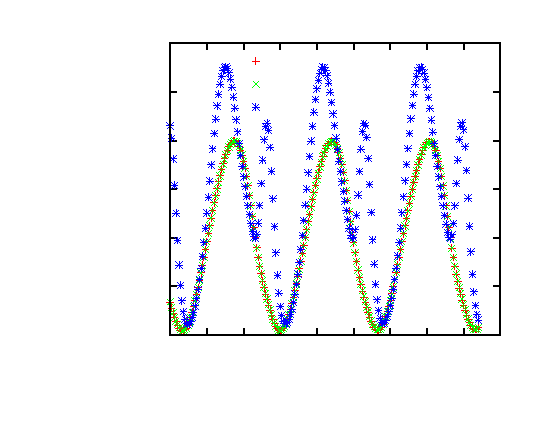
\includegraphics{dvy_cartesian_00005}}%
    \gplfronttext
  \end{picture}%
\endgroup

  % GNUPLOT: LaTeX picture with Postscript
\begingroup
  \makeatletter
  \providecommand\color[2][]{%
    \GenericError{(gnuplot) \space\space\space\@spaces}{%
      Package color not loaded in conjunction with
      terminal option `colourtext'%
    }{See the gnuplot documentation for explanation.%
    }{Either use 'blacktext' in gnuplot or load the package
      color.sty in LaTeX.}%
    \renewcommand\color[2][]{}%
  }%
  \providecommand\includegraphics[2][]{%
    \GenericError{(gnuplot) \space\space\space\@spaces}{%
      Package graphicx or graphics not loaded%
    }{See the gnuplot documentation for explanation.%
    }{The gnuplot epslatex terminal needs graphicx.sty or graphics.sty.}%
    \renewcommand\includegraphics[2][]{}%
  }%
  \providecommand\rotatebox[2]{#2}%
  \@ifundefined{ifGPcolor}{%
    \newif\ifGPcolor
    \GPcolortrue
  }{}%
  \@ifundefined{ifGPblacktext}{%
    \newif\ifGPblacktext
    \GPblacktextfalse
  }{}%
  % define a \g@addto@macro without @ in the name:
  \let\gplgaddtomacro\g@addto@macro
  % define empty templates for all commands taking text:
  \gdef\gplbacktext{}%
  \gdef\gplfronttext{}%
  \makeatother
  \ifGPblacktext
    % no textcolor at all
    \def\colorrgb#1{}%
    \def\colorgray#1{}%
  \else
    % gray or color?
    \ifGPcolor
      \def\colorrgb#1{\color[rgb]{#1}}%
      \def\colorgray#1{\color[gray]{#1}}%
      \expandafter\def\csname LTw\endcsname{\color{white}}%
      \expandafter\def\csname LTb\endcsname{\color{black}}%
      \expandafter\def\csname LTa\endcsname{\color{black}}%
      \expandafter\def\csname LT0\endcsname{\color[rgb]{1,0,0}}%
      \expandafter\def\csname LT1\endcsname{\color[rgb]{0,1,0}}%
      \expandafter\def\csname LT2\endcsname{\color[rgb]{0,0,1}}%
      \expandafter\def\csname LT3\endcsname{\color[rgb]{1,0,1}}%
      \expandafter\def\csname LT4\endcsname{\color[rgb]{0,1,1}}%
      \expandafter\def\csname LT5\endcsname{\color[rgb]{1,1,0}}%
      \expandafter\def\csname LT6\endcsname{\color[rgb]{0,0,0}}%
      \expandafter\def\csname LT7\endcsname{\color[rgb]{1,0.3,0}}%
      \expandafter\def\csname LT8\endcsname{\color[rgb]{0.5,0.5,0.5}}%
    \else
      % gray
      \def\colorrgb#1{\color{black}}%
      \def\colorgray#1{\color[gray]{#1}}%
      \expandafter\def\csname LTw\endcsname{\color{white}}%
      \expandafter\def\csname LTb\endcsname{\color{black}}%
      \expandafter\def\csname LTa\endcsname{\color{black}}%
      \expandafter\def\csname LT0\endcsname{\color{black}}%
      \expandafter\def\csname LT1\endcsname{\color{black}}%
      \expandafter\def\csname LT2\endcsname{\color{black}}%
      \expandafter\def\csname LT3\endcsname{\color{black}}%
      \expandafter\def\csname LT4\endcsname{\color{black}}%
      \expandafter\def\csname LT5\endcsname{\color{black}}%
      \expandafter\def\csname LT6\endcsname{\color{black}}%
      \expandafter\def\csname LT7\endcsname{\color{black}}%
      \expandafter\def\csname LT8\endcsname{\color{black}}%
    \fi
  \fi
  \setlength{\unitlength}{0.0500bp}%
  \begin{picture}(5040.00,3770.00)%
    \gplgaddtomacro\gplbacktext{%
      \csname LTb\endcsname%
      \put(1342,704){\makebox(0,0)[r]{\strut{}$-0.001$}}%
      \put(1342,1264){\makebox(0,0)[r]{\strut{}$-0.0005$}}%
      \put(1342,1824){\makebox(0,0)[r]{\strut{}$0$}}%
      \put(1342,2385){\makebox(0,0)[r]{\strut{}$0.0005$}}%
      \put(1342,2945){\makebox(0,0)[r]{\strut{}$0.001$}}%
      \put(1342,3505){\makebox(0,0)[r]{\strut{}$0.0015$}}%
      \put(1474,484){\makebox(0,0){\strut{}$0$}}%
      \put(1826,484){\makebox(0,0){\strut{}$50$}}%
      \put(2178,484){\makebox(0,0){\strut{}$100$}}%
      \put(2530,484){\makebox(0,0){\strut{}$150$}}%
      \put(2882,484){\makebox(0,0){\strut{}$200$}}%
      \put(3235,484){\makebox(0,0){\strut{}$250$}}%
      \put(3587,484){\makebox(0,0){\strut{}$300$}}%
      \put(3939,484){\makebox(0,0){\strut{}$350$}}%
      \put(4291,484){\makebox(0,0){\strut{}$400$}}%
      \put(4643,484){\makebox(0,0){\strut{}$450$}}%
      \put(176,2104){\rotatebox{-270}{\makebox(0,0){\strut{}$Difference (km/s)$}}}%
      \put(3058,154){\makebox(0,0){\strut{}$Minutes$}}%
    }%
    \gplgaddtomacro\gplfronttext{%
      \csname LTb\endcsname%
      \put(1870,3332){\makebox(0,0)[r]{\strut{}vl}}%
      \csname LTb\endcsname%
      \put(1870,3112){\makebox(0,0)[r]{\strut{}pn}}%
      \csname LTb\endcsname%
      \put(1870,2892){\makebox(0,0)[r]{\strut{}la}}%
    }%
    \gplbacktext
    \put(0,0){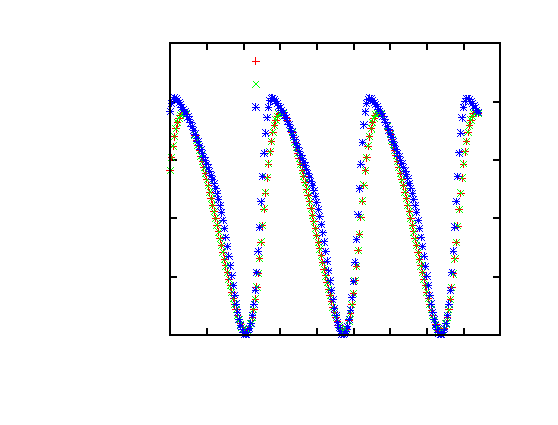
\includegraphics{dvz_cartesian_00005}}%
    \gplfronttext
  \end{picture}%
\endgroup

\caption{Difference (km/s) of SGP4Extension algorithms Lara, Vallado Long and Polar Nodals with Vallado's C++ results for TLE 00005}
\label{fig:vel05}
\end{figure}

\begin{figure}[htb]
  % GNUPLOT: LaTeX picture with Postscript
\begingroup
  \makeatletter
  \providecommand\color[2][]{%
    \GenericError{(gnuplot) \space\space\space\@spaces}{%
      Package color not loaded in conjunction with
      terminal option `colourtext'%
    }{See the gnuplot documentation for explanation.%
    }{Either use 'blacktext' in gnuplot or load the package
      color.sty in LaTeX.}%
    \renewcommand\color[2][]{}%
  }%
  \providecommand\includegraphics[2][]{%
    \GenericError{(gnuplot) \space\space\space\@spaces}{%
      Package graphicx or graphics not loaded%
    }{See the gnuplot documentation for explanation.%
    }{The gnuplot epslatex terminal needs graphicx.sty or graphics.sty.}%
    \renewcommand\includegraphics[2][]{}%
  }%
  \providecommand\rotatebox[2]{#2}%
  \@ifundefined{ifGPcolor}{%
    \newif\ifGPcolor
    \GPcolortrue
  }{}%
  \@ifundefined{ifGPblacktext}{%
    \newif\ifGPblacktext
    \GPblacktextfalse
  }{}%
  % define a \g@addto@macro without @ in the name:
  \let\gplgaddtomacro\g@addto@macro
  % define empty templates for all commands taking text:
  \gdef\gplbacktext{}%
  \gdef\gplfronttext{}%
  \makeatother
  \ifGPblacktext
    % no textcolor at all
    \def\colorrgb#1{}%
    \def\colorgray#1{}%
  \else
    % gray or color?
    \ifGPcolor
      \def\colorrgb#1{\color[rgb]{#1}}%
      \def\colorgray#1{\color[gray]{#1}}%
      \expandafter\def\csname LTw\endcsname{\color{white}}%
      \expandafter\def\csname LTb\endcsname{\color{black}}%
      \expandafter\def\csname LTa\endcsname{\color{black}}%
      \expandafter\def\csname LT0\endcsname{\color[rgb]{1,0,0}}%
      \expandafter\def\csname LT1\endcsname{\color[rgb]{0,1,0}}%
      \expandafter\def\csname LT2\endcsname{\color[rgb]{0,0,1}}%
      \expandafter\def\csname LT3\endcsname{\color[rgb]{1,0,1}}%
      \expandafter\def\csname LT4\endcsname{\color[rgb]{0,1,1}}%
      \expandafter\def\csname LT5\endcsname{\color[rgb]{1,1,0}}%
      \expandafter\def\csname LT6\endcsname{\color[rgb]{0,0,0}}%
      \expandafter\def\csname LT7\endcsname{\color[rgb]{1,0.3,0}}%
      \expandafter\def\csname LT8\endcsname{\color[rgb]{0.5,0.5,0.5}}%
    \else
      % gray
      \def\colorrgb#1{\color{black}}%
      \def\colorgray#1{\color[gray]{#1}}%
      \expandafter\def\csname LTw\endcsname{\color{white}}%
      \expandafter\def\csname LTb\endcsname{\color{black}}%
      \expandafter\def\csname LTa\endcsname{\color{black}}%
      \expandafter\def\csname LT0\endcsname{\color{black}}%
      \expandafter\def\csname LT1\endcsname{\color{black}}%
      \expandafter\def\csname LT2\endcsname{\color{black}}%
      \expandafter\def\csname LT3\endcsname{\color{black}}%
      \expandafter\def\csname LT4\endcsname{\color{black}}%
      \expandafter\def\csname LT5\endcsname{\color{black}}%
      \expandafter\def\csname LT6\endcsname{\color{black}}%
      \expandafter\def\csname LT7\endcsname{\color{black}}%
      \expandafter\def\csname LT8\endcsname{\color{black}}%
    \fi
  \fi
  \setlength{\unitlength}{0.0500bp}%
  \begin{picture}(5040.00,3770.00)%
    \gplgaddtomacro\gplbacktext{%
      \csname LTb\endcsname%
      \put(1474,704){\makebox(0,0)[r]{\strut{}$6.2e-05$}}%
      \put(1474,1104){\makebox(0,0)[r]{\strut{}$6.25e-05$}}%
      \put(1474,1504){\makebox(0,0)[r]{\strut{}$6.3e-05$}}%
      \put(1474,1904){\makebox(0,0)[r]{\strut{}$6.35e-05$}}%
      \put(1474,2305){\makebox(0,0)[r]{\strut{}$6.4e-05$}}%
      \put(1474,2705){\makebox(0,0)[r]{\strut{}$6.45e-05$}}%
      \put(1474,3105){\makebox(0,0)[r]{\strut{}$6.5e-05$}}%
      \put(1474,3505){\makebox(0,0)[r]{\strut{}$6.55e-05$}}%
      \put(1606,484){\makebox(0,0){\strut{}$0$}}%
      \put(1943,484){\makebox(0,0){\strut{}$50$}}%
      \put(2281,484){\makebox(0,0){\strut{}$100$}}%
      \put(2618,484){\makebox(0,0){\strut{}$150$}}%
      \put(2956,484){\makebox(0,0){\strut{}$200$}}%
      \put(3293,484){\makebox(0,0){\strut{}$250$}}%
      \put(3631,484){\makebox(0,0){\strut{}$300$}}%
      \put(3968,484){\makebox(0,0){\strut{}$350$}}%
      \put(4306,484){\makebox(0,0){\strut{}$400$}}%
      \put(4643,484){\makebox(0,0){\strut{}$450$}}%
      \put(176,2104){\rotatebox{-270}{\makebox(0,0){\strut{}Difference}}}%
      \put(3124,154){\makebox(0,0){\strut{}$Minutes$}}%
    }%
    \gplgaddtomacro\gplfronttext{%
      \csname LTb\endcsname%
      \put(2002,3332){\makebox(0,0)[r]{\strut{}vl}}%
      \csname LTb\endcsname%
      \put(2002,3112){\makebox(0,0)[r]{\strut{}pn}}%
      \csname LTb\endcsname%
      \put(2002,2892){\makebox(0,0)[r]{\strut{}la}}%
    }%
    \gplbacktext
    \put(0,0){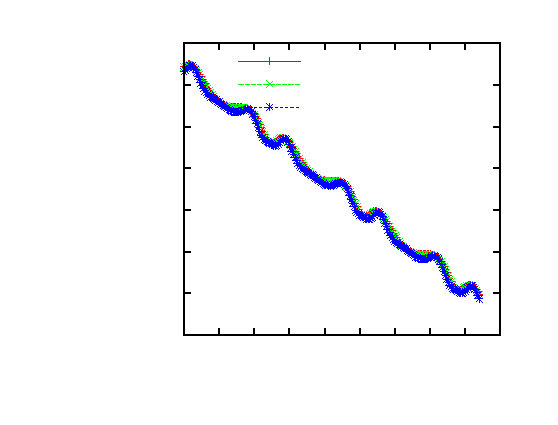
\includegraphics{dI_pn_00005}}%
    \gplfronttext
  \end{picture}%
\endgroup

  % GNUPLOT: LaTeX picture with Postscript
\begingroup
  \makeatletter
  \providecommand\color[2][]{%
    \GenericError{(gnuplot) \space\space\space\@spaces}{%
      Package color not loaded in conjunction with
      terminal option `colourtext'%
    }{See the gnuplot documentation for explanation.%
    }{Either use 'blacktext' in gnuplot or load the package
      color.sty in LaTeX.}%
    \renewcommand\color[2][]{}%
  }%
  \providecommand\includegraphics[2][]{%
    \GenericError{(gnuplot) \space\space\space\@spaces}{%
      Package graphicx or graphics not loaded%
    }{See the gnuplot documentation for explanation.%
    }{The gnuplot epslatex terminal needs graphicx.sty or graphics.sty.}%
    \renewcommand\includegraphics[2][]{}%
  }%
  \providecommand\rotatebox[2]{#2}%
  \@ifundefined{ifGPcolor}{%
    \newif\ifGPcolor
    \GPcolortrue
  }{}%
  \@ifundefined{ifGPblacktext}{%
    \newif\ifGPblacktext
    \GPblacktextfalse
  }{}%
  % define a \g@addto@macro without @ in the name:
  \let\gplgaddtomacro\g@addto@macro
  % define empty templates for all commands taking text:
  \gdef\gplbacktext{}%
  \gdef\gplfronttext{}%
  \makeatother
  \ifGPblacktext
    % no textcolor at all
    \def\colorrgb#1{}%
    \def\colorgray#1{}%
  \else
    % gray or color?
    \ifGPcolor
      \def\colorrgb#1{\color[rgb]{#1}}%
      \def\colorgray#1{\color[gray]{#1}}%
      \expandafter\def\csname LTw\endcsname{\color{white}}%
      \expandafter\def\csname LTb\endcsname{\color{black}}%
      \expandafter\def\csname LTa\endcsname{\color{black}}%
      \expandafter\def\csname LT0\endcsname{\color[rgb]{1,0,0}}%
      \expandafter\def\csname LT1\endcsname{\color[rgb]{0,1,0}}%
      \expandafter\def\csname LT2\endcsname{\color[rgb]{0,0,1}}%
      \expandafter\def\csname LT3\endcsname{\color[rgb]{1,0,1}}%
      \expandafter\def\csname LT4\endcsname{\color[rgb]{0,1,1}}%
      \expandafter\def\csname LT5\endcsname{\color[rgb]{1,1,0}}%
      \expandafter\def\csname LT6\endcsname{\color[rgb]{0,0,0}}%
      \expandafter\def\csname LT7\endcsname{\color[rgb]{1,0.3,0}}%
      \expandafter\def\csname LT8\endcsname{\color[rgb]{0.5,0.5,0.5}}%
    \else
      % gray
      \def\colorrgb#1{\color{black}}%
      \def\colorgray#1{\color[gray]{#1}}%
      \expandafter\def\csname LTw\endcsname{\color{white}}%
      \expandafter\def\csname LTb\endcsname{\color{black}}%
      \expandafter\def\csname LTa\endcsname{\color{black}}%
      \expandafter\def\csname LT0\endcsname{\color{black}}%
      \expandafter\def\csname LT1\endcsname{\color{black}}%
      \expandafter\def\csname LT2\endcsname{\color{black}}%
      \expandafter\def\csname LT3\endcsname{\color{black}}%
      \expandafter\def\csname LT4\endcsname{\color{black}}%
      \expandafter\def\csname LT5\endcsname{\color{black}}%
      \expandafter\def\csname LT6\endcsname{\color{black}}%
      \expandafter\def\csname LT7\endcsname{\color{black}}%
      \expandafter\def\csname LT8\endcsname{\color{black}}%
    \fi
  \fi
  \setlength{\unitlength}{0.0500bp}%
  \begin{picture}(5040.00,3770.00)%
    \gplgaddtomacro\gplbacktext{%
      \csname LTb\endcsname%
      \put(1606,704){\makebox(0,0)[r]{\strut{}$-0.00025$}}%
      \put(1606,959){\makebox(0,0)[r]{\strut{}$-0.000245$}}%
      \put(1606,1213){\makebox(0,0)[r]{\strut{}$-0.00024$}}%
      \put(1606,1468){\makebox(0,0)[r]{\strut{}$-0.000235$}}%
      \put(1606,1723){\makebox(0,0)[r]{\strut{}$-0.00023$}}%
      \put(1606,1977){\makebox(0,0)[r]{\strut{}$-0.000225$}}%
      \put(1606,2232){\makebox(0,0)[r]{\strut{}$-0.00022$}}%
      \put(1606,2486){\makebox(0,0)[r]{\strut{}$-0.000215$}}%
      \put(1606,2741){\makebox(0,0)[r]{\strut{}$-0.00021$}}%
      \put(1606,2996){\makebox(0,0)[r]{\strut{}$-0.000205$}}%
      \put(1606,3250){\makebox(0,0)[r]{\strut{}$-0.0002$}}%
      \put(1606,3505){\makebox(0,0)[r]{\strut{}$-0.000195$}}%
      \put(1738,484){\makebox(0,0){\strut{}$0$}}%
      \put(2061,484){\makebox(0,0){\strut{}$50$}}%
      \put(2384,484){\makebox(0,0){\strut{}$100$}}%
      \put(2706,484){\makebox(0,0){\strut{}$150$}}%
      \put(3029,484){\makebox(0,0){\strut{}$200$}}%
      \put(3352,484){\makebox(0,0){\strut{}$250$}}%
      \put(3675,484){\makebox(0,0){\strut{}$300$}}%
      \put(3997,484){\makebox(0,0){\strut{}$350$}}%
      \put(4320,484){\makebox(0,0){\strut{}$400$}}%
      \put(4643,484){\makebox(0,0){\strut{}$450$}}%
      \put(176,2104){\rotatebox{-270}{\makebox(0,0){\strut{}Difference}}}%
      \put(3190,154){\makebox(0,0){\strut{}$Minutes$}}%
    }%
    \gplgaddtomacro\gplfronttext{%
      \csname LTb\endcsname%
      \put(2134,3332){\makebox(0,0)[r]{\strut{}vl}}%
      \csname LTb\endcsname%
      \put(2134,3112){\makebox(0,0)[r]{\strut{}pn}}%
      \csname LTb\endcsname%
      \put(2134,2892){\makebox(0,0)[r]{\strut{}la}}%
    }%
    \gplbacktext
    \put(0,0){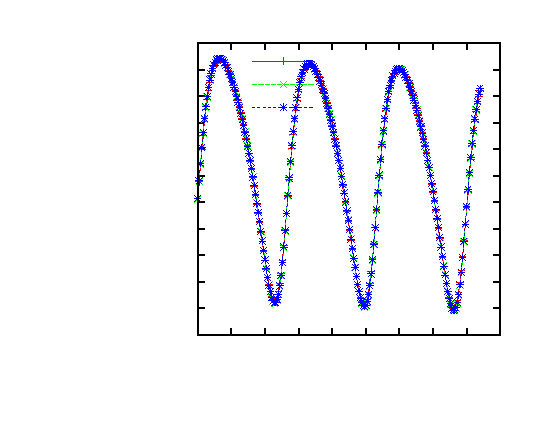
\includegraphics{dθ_pn_00005}}%
    \gplfronttext
  \end{picture}%
\endgroup

  % GNUPLOT: LaTeX picture with Postscript
\begingroup
  \makeatletter
  \providecommand\color[2][]{%
    \GenericError{(gnuplot) \space\space\space\@spaces}{%
      Package color not loaded in conjunction with
      terminal option `colourtext'%
    }{See the gnuplot documentation for explanation.%
    }{Either use 'blacktext' in gnuplot or load the package
      color.sty in LaTeX.}%
    \renewcommand\color[2][]{}%
  }%
  \providecommand\includegraphics[2][]{%
    \GenericError{(gnuplot) \space\space\space\@spaces}{%
      Package graphicx or graphics not loaded%
    }{See the gnuplot documentation for explanation.%
    }{The gnuplot epslatex terminal needs graphicx.sty or graphics.sty.}%
    \renewcommand\includegraphics[2][]{}%
  }%
  \providecommand\rotatebox[2]{#2}%
  \@ifundefined{ifGPcolor}{%
    \newif\ifGPcolor
    \GPcolortrue
  }{}%
  \@ifundefined{ifGPblacktext}{%
    \newif\ifGPblacktext
    \GPblacktextfalse
  }{}%
  % define a \g@addto@macro without @ in the name:
  \let\gplgaddtomacro\g@addto@macro
  % define empty templates for all commands taking text:
  \gdef\gplbacktext{}%
  \gdef\gplfronttext{}%
  \makeatother
  \ifGPblacktext
    % no textcolor at all
    \def\colorrgb#1{}%
    \def\colorgray#1{}%
  \else
    % gray or color?
    \ifGPcolor
      \def\colorrgb#1{\color[rgb]{#1}}%
      \def\colorgray#1{\color[gray]{#1}}%
      \expandafter\def\csname LTw\endcsname{\color{white}}%
      \expandafter\def\csname LTb\endcsname{\color{black}}%
      \expandafter\def\csname LTa\endcsname{\color{black}}%
      \expandafter\def\csname LT0\endcsname{\color[rgb]{1,0,0}}%
      \expandafter\def\csname LT1\endcsname{\color[rgb]{0,1,0}}%
      \expandafter\def\csname LT2\endcsname{\color[rgb]{0,0,1}}%
      \expandafter\def\csname LT3\endcsname{\color[rgb]{1,0,1}}%
      \expandafter\def\csname LT4\endcsname{\color[rgb]{0,1,1}}%
      \expandafter\def\csname LT5\endcsname{\color[rgb]{1,1,0}}%
      \expandafter\def\csname LT6\endcsname{\color[rgb]{0,0,0}}%
      \expandafter\def\csname LT7\endcsname{\color[rgb]{1,0.3,0}}%
      \expandafter\def\csname LT8\endcsname{\color[rgb]{0.5,0.5,0.5}}%
    \else
      % gray
      \def\colorrgb#1{\color{black}}%
      \def\colorgray#1{\color[gray]{#1}}%
      \expandafter\def\csname LTw\endcsname{\color{white}}%
      \expandafter\def\csname LTb\endcsname{\color{black}}%
      \expandafter\def\csname LTa\endcsname{\color{black}}%
      \expandafter\def\csname LT0\endcsname{\color{black}}%
      \expandafter\def\csname LT1\endcsname{\color{black}}%
      \expandafter\def\csname LT2\endcsname{\color{black}}%
      \expandafter\def\csname LT3\endcsname{\color{black}}%
      \expandafter\def\csname LT4\endcsname{\color{black}}%
      \expandafter\def\csname LT5\endcsname{\color{black}}%
      \expandafter\def\csname LT6\endcsname{\color{black}}%
      \expandafter\def\csname LT7\endcsname{\color{black}}%
      \expandafter\def\csname LT8\endcsname{\color{black}}%
    \fi
  \fi
  \setlength{\unitlength}{0.0500bp}%
  \begin{picture}(5040.00,3770.00)%
    \gplgaddtomacro\gplbacktext{%
      \csname LTb\endcsname%
      \put(1606,704){\makebox(0,0)[r]{\strut{}$0.000215$}}%
      \put(1606,1104){\makebox(0,0)[r]{\strut{}$0.0002155$}}%
      \put(1606,1504){\makebox(0,0)[r]{\strut{}$0.000216$}}%
      \put(1606,1904){\makebox(0,0)[r]{\strut{}$0.0002165$}}%
      \put(1606,2305){\makebox(0,0)[r]{\strut{}$0.000217$}}%
      \put(1606,2705){\makebox(0,0)[r]{\strut{}$0.0002175$}}%
      \put(1606,3105){\makebox(0,0)[r]{\strut{}$0.000218$}}%
      \put(1606,3505){\makebox(0,0)[r]{\strut{}$0.0002185$}}%
      \put(1738,484){\makebox(0,0){\strut{}$0$}}%
      \put(2061,484){\makebox(0,0){\strut{}$50$}}%
      \put(2384,484){\makebox(0,0){\strut{}$100$}}%
      \put(2706,484){\makebox(0,0){\strut{}$150$}}%
      \put(3029,484){\makebox(0,0){\strut{}$200$}}%
      \put(3352,484){\makebox(0,0){\strut{}$250$}}%
      \put(3675,484){\makebox(0,0){\strut{}$300$}}%
      \put(3997,484){\makebox(0,0){\strut{}$350$}}%
      \put(4320,484){\makebox(0,0){\strut{}$400$}}%
      \put(4643,484){\makebox(0,0){\strut{}$450$}}%
      \put(176,2104){\rotatebox{-270}{\makebox(0,0){\strut{}Difference}}}%
      \put(3190,154){\makebox(0,0){\strut{}$Minutes$}}%
    }%
    \gplgaddtomacro\gplfronttext{%
      \csname LTb\endcsname%
      \put(2134,3332){\makebox(0,0)[r]{\strut{}vl}}%
      \csname LTb\endcsname%
      \put(2134,3112){\makebox(0,0)[r]{\strut{}pn}}%
      \csname LTb\endcsname%
      \put(2134,2892){\makebox(0,0)[r]{\strut{}la}}%
    }%
    \gplbacktext
    \put(0,0){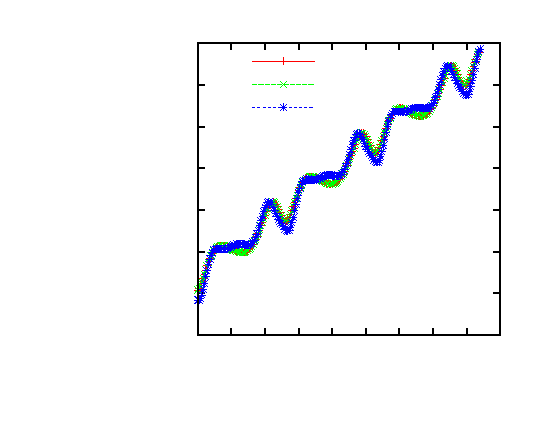
\includegraphics{dΩ_pn_00005}}%
    \gplfronttext
  \end{picture}%
\endgroup

\caption{Difference (radians) of SGP4Extension algorithms Lara, Vallado Long and Polar Nodals with Vallado's C++ results for TLE 00005}
\label{fig:arg05}
\end{figure}

\begin{figure}[htb]
  % GNUPLOT: LaTeX picture with Postscript
\begingroup
  \makeatletter
  \providecommand\color[2][]{%
    \GenericError{(gnuplot) \space\space\space\@spaces}{%
      Package color not loaded in conjunction with
      terminal option `colourtext'%
    }{See the gnuplot documentation for explanation.%
    }{Either use 'blacktext' in gnuplot or load the package
      color.sty in LaTeX.}%
    \renewcommand\color[2][]{}%
  }%
  \providecommand\includegraphics[2][]{%
    \GenericError{(gnuplot) \space\space\space\@spaces}{%
      Package graphicx or graphics not loaded%
    }{See the gnuplot documentation for explanation.%
    }{The gnuplot epslatex terminal needs graphicx.sty or graphics.sty.}%
    \renewcommand\includegraphics[2][]{}%
  }%
  \providecommand\rotatebox[2]{#2}%
  \@ifundefined{ifGPcolor}{%
    \newif\ifGPcolor
    \GPcolortrue
  }{}%
  \@ifundefined{ifGPblacktext}{%
    \newif\ifGPblacktext
    \GPblacktextfalse
  }{}%
  % define a \g@addto@macro without @ in the name:
  \let\gplgaddtomacro\g@addto@macro
  % define empty templates for all commands taking text:
  \gdef\gplbacktext{}%
  \gdef\gplfronttext{}%
  \makeatother
  \ifGPblacktext
    % no textcolor at all
    \def\colorrgb#1{}%
    \def\colorgray#1{}%
  \else
    % gray or color?
    \ifGPcolor
      \def\colorrgb#1{\color[rgb]{#1}}%
      \def\colorgray#1{\color[gray]{#1}}%
      \expandafter\def\csname LTw\endcsname{\color{white}}%
      \expandafter\def\csname LTb\endcsname{\color{black}}%
      \expandafter\def\csname LTa\endcsname{\color{black}}%
      \expandafter\def\csname LT0\endcsname{\color[rgb]{1,0,0}}%
      \expandafter\def\csname LT1\endcsname{\color[rgb]{0,1,0}}%
      \expandafter\def\csname LT2\endcsname{\color[rgb]{0,0,1}}%
      \expandafter\def\csname LT3\endcsname{\color[rgb]{1,0,1}}%
      \expandafter\def\csname LT4\endcsname{\color[rgb]{0,1,1}}%
      \expandafter\def\csname LT5\endcsname{\color[rgb]{1,1,0}}%
      \expandafter\def\csname LT6\endcsname{\color[rgb]{0,0,0}}%
      \expandafter\def\csname LT7\endcsname{\color[rgb]{1,0.3,0}}%
      \expandafter\def\csname LT8\endcsname{\color[rgb]{0.5,0.5,0.5}}%
    \else
      % gray
      \def\colorrgb#1{\color{black}}%
      \def\colorgray#1{\color[gray]{#1}}%
      \expandafter\def\csname LTw\endcsname{\color{white}}%
      \expandafter\def\csname LTb\endcsname{\color{black}}%
      \expandafter\def\csname LTa\endcsname{\color{black}}%
      \expandafter\def\csname LT0\endcsname{\color{black}}%
      \expandafter\def\csname LT1\endcsname{\color{black}}%
      \expandafter\def\csname LT2\endcsname{\color{black}}%
      \expandafter\def\csname LT3\endcsname{\color{black}}%
      \expandafter\def\csname LT4\endcsname{\color{black}}%
      \expandafter\def\csname LT5\endcsname{\color{black}}%
      \expandafter\def\csname LT6\endcsname{\color{black}}%
      \expandafter\def\csname LT7\endcsname{\color{black}}%
      \expandafter\def\csname LT8\endcsname{\color{black}}%
    \fi
  \fi
  \setlength{\unitlength}{0.0500bp}%
  \begin{picture}(5040.00,3770.00)%
    \gplgaddtomacro\gplbacktext{%
      \csname LTb\endcsname%
      \put(1474,704){\makebox(0,0)[r]{\strut{}$-3.5e-05$}}%
      \put(1474,984){\makebox(0,0)[r]{\strut{}$-3e-05$}}%
      \put(1474,1264){\makebox(0,0)[r]{\strut{}$-2.5e-05$}}%
      \put(1474,1544){\makebox(0,0)[r]{\strut{}$-2e-05$}}%
      \put(1474,1824){\makebox(0,0)[r]{\strut{}$-1.5e-05$}}%
      \put(1474,2105){\makebox(0,0)[r]{\strut{}$-1e-05$}}%
      \put(1474,2385){\makebox(0,0)[r]{\strut{}$-5e-06$}}%
      \put(1474,2665){\makebox(0,0)[r]{\strut{}$0$}}%
      \put(1474,2945){\makebox(0,0)[r]{\strut{}$5e-06$}}%
      \put(1474,3225){\makebox(0,0)[r]{\strut{}$1e-05$}}%
      \put(1474,3505){\makebox(0,0)[r]{\strut{}$1.5e-05$}}%
      \put(1606,484){\makebox(0,0){\strut{}$0$}}%
      \put(1943,484){\makebox(0,0){\strut{}$50$}}%
      \put(2281,484){\makebox(0,0){\strut{}$100$}}%
      \put(2618,484){\makebox(0,0){\strut{}$150$}}%
      \put(2956,484){\makebox(0,0){\strut{}$200$}}%
      \put(3293,484){\makebox(0,0){\strut{}$250$}}%
      \put(3631,484){\makebox(0,0){\strut{}$300$}}%
      \put(3968,484){\makebox(0,0){\strut{}$350$}}%
      \put(4306,484){\makebox(0,0){\strut{}$400$}}%
      \put(4643,484){\makebox(0,0){\strut{}$450$}}%
      \put(176,2104){\rotatebox{-270}{\makebox(0,0){\strut{}Difference}}}%
      \put(3124,154){\makebox(0,0){\strut{}$Minutes$}}%
    }%
    \gplgaddtomacro\gplfronttext{%
      \csname LTb\endcsname%
      \put(2002,3332){\makebox(0,0)[r]{\strut{}vl}}%
      \csname LTb\endcsname%
      \put(2002,3112){\makebox(0,0)[r]{\strut{}pn}}%
      \csname LTb\endcsname%
      \put(2002,2892){\makebox(0,0)[r]{\strut{}la}}%
    }%
    \gplbacktext
    \put(0,0){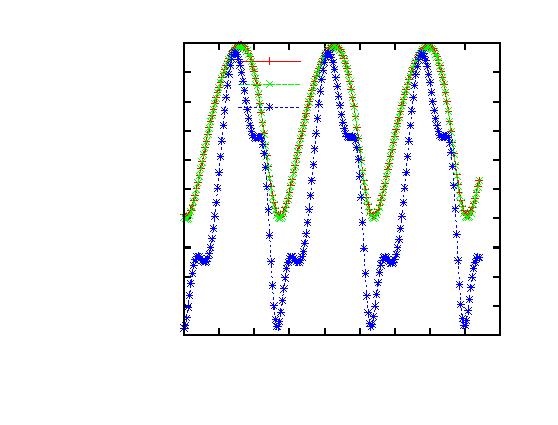
\includegraphics{dr_pn_00005}}%
    \gplfronttext
  \end{picture}%
\endgroup

  % GNUPLOT: LaTeX picture with Postscript
\begingroup
  \makeatletter
  \providecommand\color[2][]{%
    \GenericError{(gnuplot) \space\space\space\@spaces}{%
      Package color not loaded in conjunction with
      terminal option `colourtext'%
    }{See the gnuplot documentation for explanation.%
    }{Either use 'blacktext' in gnuplot or load the package
      color.sty in LaTeX.}%
    \renewcommand\color[2][]{}%
  }%
  \providecommand\includegraphics[2][]{%
    \GenericError{(gnuplot) \space\space\space\@spaces}{%
      Package graphicx or graphics not loaded%
    }{See the gnuplot documentation for explanation.%
    }{The gnuplot epslatex terminal needs graphicx.sty or graphics.sty.}%
    \renewcommand\includegraphics[2][]{}%
  }%
  \providecommand\rotatebox[2]{#2}%
  \@ifundefined{ifGPcolor}{%
    \newif\ifGPcolor
    \GPcolortrue
  }{}%
  \@ifundefined{ifGPblacktext}{%
    \newif\ifGPblacktext
    \GPblacktextfalse
  }{}%
  % define a \g@addto@macro without @ in the name:
  \let\gplgaddtomacro\g@addto@macro
  % define empty templates for all commands taking text:
  \gdef\gplbacktext{}%
  \gdef\gplfronttext{}%
  \makeatother
  \ifGPblacktext
    % no textcolor at all
    \def\colorrgb#1{}%
    \def\colorgray#1{}%
  \else
    % gray or color?
    \ifGPcolor
      \def\colorrgb#1{\color[rgb]{#1}}%
      \def\colorgray#1{\color[gray]{#1}}%
      \expandafter\def\csname LTw\endcsname{\color{white}}%
      \expandafter\def\csname LTb\endcsname{\color{black}}%
      \expandafter\def\csname LTa\endcsname{\color{black}}%
      \expandafter\def\csname LT0\endcsname{\color[rgb]{1,0,0}}%
      \expandafter\def\csname LT1\endcsname{\color[rgb]{0,1,0}}%
      \expandafter\def\csname LT2\endcsname{\color[rgb]{0,0,1}}%
      \expandafter\def\csname LT3\endcsname{\color[rgb]{1,0,1}}%
      \expandafter\def\csname LT4\endcsname{\color[rgb]{0,1,1}}%
      \expandafter\def\csname LT5\endcsname{\color[rgb]{1,1,0}}%
      \expandafter\def\csname LT6\endcsname{\color[rgb]{0,0,0}}%
      \expandafter\def\csname LT7\endcsname{\color[rgb]{1,0.3,0}}%
      \expandafter\def\csname LT8\endcsname{\color[rgb]{0.5,0.5,0.5}}%
    \else
      % gray
      \def\colorrgb#1{\color{black}}%
      \def\colorgray#1{\color[gray]{#1}}%
      \expandafter\def\csname LTw\endcsname{\color{white}}%
      \expandafter\def\csname LTb\endcsname{\color{black}}%
      \expandafter\def\csname LTa\endcsname{\color{black}}%
      \expandafter\def\csname LT0\endcsname{\color{black}}%
      \expandafter\def\csname LT1\endcsname{\color{black}}%
      \expandafter\def\csname LT2\endcsname{\color{black}}%
      \expandafter\def\csname LT3\endcsname{\color{black}}%
      \expandafter\def\csname LT4\endcsname{\color{black}}%
      \expandafter\def\csname LT5\endcsname{\color{black}}%
      \expandafter\def\csname LT6\endcsname{\color{black}}%
      \expandafter\def\csname LT7\endcsname{\color{black}}%
      \expandafter\def\csname LT8\endcsname{\color{black}}%
    \fi
  \fi
  \setlength{\unitlength}{0.0500bp}%
  \begin{picture}(5040.00,3770.00)%
    \gplgaddtomacro\gplbacktext{%
      \csname LTb\endcsname%
      \put(1474,704){\makebox(0,0)[r]{\strut{}$-1.5e-05$}}%
      \put(1474,1264){\makebox(0,0)[r]{\strut{}$-1e-05$}}%
      \put(1474,1824){\makebox(0,0)[r]{\strut{}$-5e-06$}}%
      \put(1474,2385){\makebox(0,0)[r]{\strut{}$0$}}%
      \put(1474,2945){\makebox(0,0)[r]{\strut{}$5e-06$}}%
      \put(1474,3505){\makebox(0,0)[r]{\strut{}$1e-05$}}%
      \put(1606,484){\makebox(0,0){\strut{}$0$}}%
      \put(1943,484){\makebox(0,0){\strut{}$50$}}%
      \put(2281,484){\makebox(0,0){\strut{}$100$}}%
      \put(2618,484){\makebox(0,0){\strut{}$150$}}%
      \put(2956,484){\makebox(0,0){\strut{}$200$}}%
      \put(3293,484){\makebox(0,0){\strut{}$250$}}%
      \put(3631,484){\makebox(0,0){\strut{}$300$}}%
      \put(3968,484){\makebox(0,0){\strut{}$350$}}%
      \put(4306,484){\makebox(0,0){\strut{}$400$}}%
      \put(4643,484){\makebox(0,0){\strut{}$450$}}%
      \put(176,2104){\rotatebox{-270}{\makebox(0,0){\strut{}Difference}}}%
      \put(3124,154){\makebox(0,0){\strut{}$Minutes$}}%
    }%
    \gplgaddtomacro\gplfronttext{%
      \csname LTb\endcsname%
      \put(2002,3332){\makebox(0,0)[r]{\strut{}vl}}%
      \csname LTb\endcsname%
      \put(2002,3112){\makebox(0,0)[r]{\strut{}pn}}%
      \csname LTb\endcsname%
      \put(2002,2892){\makebox(0,0)[r]{\strut{}la}}%
    }%
    \gplbacktext
    \put(0,0){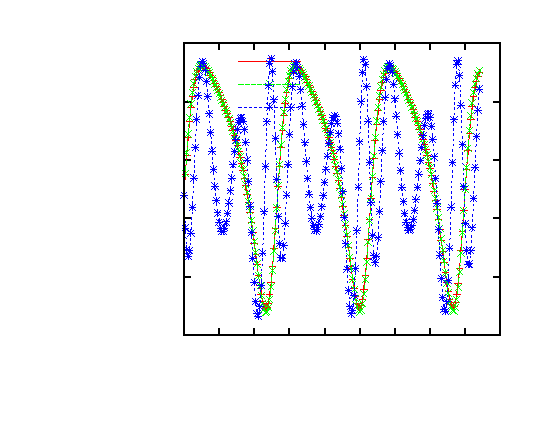
\includegraphics{dRV_pn_00005}}%
    \gplfronttext
  \end{picture}%
\endgroup

  % GNUPLOT: LaTeX picture with Postscript
\begingroup
  \makeatletter
  \providecommand\color[2][]{%
    \GenericError{(gnuplot) \space\space\space\@spaces}{%
      Package color not loaded in conjunction with
      terminal option `colourtext'%
    }{See the gnuplot documentation for explanation.%
    }{Either use 'blacktext' in gnuplot or load the package
      color.sty in LaTeX.}%
    \renewcommand\color[2][]{}%
  }%
  \providecommand\includegraphics[2][]{%
    \GenericError{(gnuplot) \space\space\space\@spaces}{%
      Package graphicx or graphics not loaded%
    }{See the gnuplot documentation for explanation.%
    }{The gnuplot epslatex terminal needs graphicx.sty or graphics.sty.}%
    \renewcommand\includegraphics[2][]{}%
  }%
  \providecommand\rotatebox[2]{#2}%
  \@ifundefined{ifGPcolor}{%
    \newif\ifGPcolor
    \GPcolortrue
  }{}%
  \@ifundefined{ifGPblacktext}{%
    \newif\ifGPblacktext
    \GPblacktextfalse
  }{}%
  % define a \g@addto@macro without @ in the name:
  \let\gplgaddtomacro\g@addto@macro
  % define empty templates for all commands taking text:
  \gdef\gplbacktext{}%
  \gdef\gplfronttext{}%
  \makeatother
  \ifGPblacktext
    % no textcolor at all
    \def\colorrgb#1{}%
    \def\colorgray#1{}%
  \else
    % gray or color?
    \ifGPcolor
      \def\colorrgb#1{\color[rgb]{#1}}%
      \def\colorgray#1{\color[gray]{#1}}%
      \expandafter\def\csname LTw\endcsname{\color{white}}%
      \expandafter\def\csname LTb\endcsname{\color{black}}%
      \expandafter\def\csname LTa\endcsname{\color{black}}%
      \expandafter\def\csname LT0\endcsname{\color[rgb]{1,0,0}}%
      \expandafter\def\csname LT1\endcsname{\color[rgb]{0,1,0}}%
      \expandafter\def\csname LT2\endcsname{\color[rgb]{0,0,1}}%
      \expandafter\def\csname LT3\endcsname{\color[rgb]{1,0,1}}%
      \expandafter\def\csname LT4\endcsname{\color[rgb]{0,1,1}}%
      \expandafter\def\csname LT5\endcsname{\color[rgb]{1,1,0}}%
      \expandafter\def\csname LT6\endcsname{\color[rgb]{0,0,0}}%
      \expandafter\def\csname LT7\endcsname{\color[rgb]{1,0.3,0}}%
      \expandafter\def\csname LT8\endcsname{\color[rgb]{0.5,0.5,0.5}}%
    \else
      % gray
      \def\colorrgb#1{\color{black}}%
      \def\colorgray#1{\color[gray]{#1}}%
      \expandafter\def\csname LTw\endcsname{\color{white}}%
      \expandafter\def\csname LTb\endcsname{\color{black}}%
      \expandafter\def\csname LTa\endcsname{\color{black}}%
      \expandafter\def\csname LT0\endcsname{\color{black}}%
      \expandafter\def\csname LT1\endcsname{\color{black}}%
      \expandafter\def\csname LT2\endcsname{\color{black}}%
      \expandafter\def\csname LT3\endcsname{\color{black}}%
      \expandafter\def\csname LT4\endcsname{\color{black}}%
      \expandafter\def\csname LT5\endcsname{\color{black}}%
      \expandafter\def\csname LT6\endcsname{\color{black}}%
      \expandafter\def\csname LT7\endcsname{\color{black}}%
      \expandafter\def\csname LT8\endcsname{\color{black}}%
    \fi
  \fi
  \setlength{\unitlength}{0.0500bp}%
  \begin{picture}(5040.00,3770.00)%
    \gplgaddtomacro\gplbacktext{%
      \csname LTb\endcsname%
      \put(1342,704){\makebox(0,0)[r]{\strut{}$-0.0001$}}%
      \put(1342,1264){\makebox(0,0)[r]{\strut{}$-5e-05$}}%
      \put(1342,1824){\makebox(0,0)[r]{\strut{}$0$}}%
      \put(1342,2385){\makebox(0,0)[r]{\strut{}$5e-05$}}%
      \put(1342,2945){\makebox(0,0)[r]{\strut{}$0.0001$}}%
      \put(1342,3505){\makebox(0,0)[r]{\strut{}$0.00015$}}%
      \put(1474,484){\makebox(0,0){\strut{}$0$}}%
      \put(1826,484){\makebox(0,0){\strut{}$50$}}%
      \put(2178,484){\makebox(0,0){\strut{}$100$}}%
      \put(2530,484){\makebox(0,0){\strut{}$150$}}%
      \put(2882,484){\makebox(0,0){\strut{}$200$}}%
      \put(3235,484){\makebox(0,0){\strut{}$250$}}%
      \put(3587,484){\makebox(0,0){\strut{}$300$}}%
      \put(3939,484){\makebox(0,0){\strut{}$350$}}%
      \put(4291,484){\makebox(0,0){\strut{}$400$}}%
      \put(4643,484){\makebox(0,0){\strut{}$450$}}%
      \put(176,2104){\rotatebox{-270}{\makebox(0,0){\strut{}Difference}}}%
      \put(3058,154){\makebox(0,0){\strut{}$Minutes$}}%
    }%
    \gplgaddtomacro\gplfronttext{%
      \csname LTb\endcsname%
      \put(1870,3332){\makebox(0,0)[r]{\strut{}vl}}%
      \csname LTb\endcsname%
      \put(1870,3112){\makebox(0,0)[r]{\strut{}pn}}%
      \csname LTb\endcsname%
      \put(1870,2892){\makebox(0,0)[r]{\strut{}la}}%
    }%
    \gplbacktext
    \put(0,0){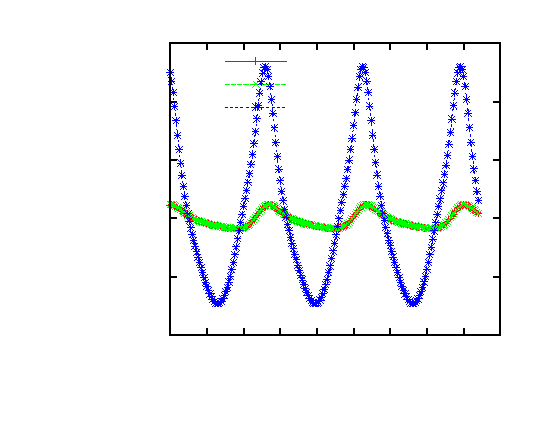
\includegraphics{drθdot_pn_00005}}%
    \gplfronttext
  \end{picture}%
\endgroup

\caption{Difference for r, radial velocity and angular momentum from SGP4Extension algorithms Lara, Vallado Long and Polar Nodals with Vallado's C++ results for TLE 00005}
\label{fig:rv05}
\end{figure}


\section{APPLICATIONS}
\label{sec:applications}
SGP4Extensions produces the same results as other SGP4 implementations.
Its interest resides in the flexibility to introduce and test new ideas related to SGP4 itself.
As example when doing conjunction analysis for space debris, the user has the possibility to design
filter algorithms based on results obtained in polar nodal variables without
the need to obtain cartesian values. One possibility when comparing two objects
is to find out the crossing points of the orbital planes and then estimate the passing times
at those points with the true anomaly \cite[sec. 9.6]{Aba2012}.

As concerns like errors and uncertainties have also to be taken into account when designing these
algorithms, more special numeric types related to Intervals can be introduced to automatically
calculate such uncertainties with the normal conjunction algorithm.

For other filter possibilities, the cartesian values can be easily obtained on demand, saving computational time and memory requirements.

Regarding speed optimizations in the current SGP4 code, when doing conjunction analysis most of the computational time goes into finding the points of close approach. Therefore, speed optimizations at SGP4 level might not have a significant impact compared with the actual design of the conjunction analysis strategy.


\section{CONCLUSIONS}
\label{sec:conclusions}

A new implementation of the SGP4 algorithm in scala is available for the community.
It provides implementations of the models using a unicode notation resembling the
actual descriptions of the models in the literature. It also allows to easily
introduce alternative models and variables related to the theory.
The software is designed for parallelization and for fine grain access to the data generated by
the propagation steps. This provides an
interesting base for massive conjunction analysis tasks.

% Figures, tables and equations must be numbered and placed within the designated margins. They may span the two
% columns. Every figure and table must also be captioned.

% If possible, position illustrations at the top of columns, rather than in the middle or at the bottom. Figure~\ref{fig:res} shows how to include images.

% For tables, the example on how they shall be captioned and formatted is provided in Table~\ref{tab:res}.


% To start a new column (but not a new page) and help balance the last-page
% column length use \vfill\pagebreak.
% -------------------------------------------------------------------------

\bibliographystyle{IEEEbib}
\bibliography{refs}

% References should be produced using the bibtex program from suitable
% BiBTeX files (here: refs). The IEEEbib.bst bibliography
% style file from IEEE produces unsorted bibliography list.
% -------------------------------------------------------------------------

\end{document}
